\chapter{Empirical Analysis}
\label{chap:empirical}
\lhead{Chapter 4. \emph{Empirical Analysis}}

\section{Data and Methodology}
This analysis aims to evaluate the performance characteristics of the GMM and KDE portfolios and compare them to those of the standard strategies. To do so, we compare the out-of-sample performance of these strategies when deployed on the S\&P500, FTSE100, STOXX50, and the HSI indices. We also perform tests on the subsets of these indices to see whether the performance characteristics are affected by the number of assets in the portfolio. To this end, we attempt every combination of the following meta-parameters:
\begin{itemize}
\item \textbf{Data frequency:} daily, weekly, monthly
\item \textbf{Portfolio rebalancing frequency:} monthly, annual
\item \textbf{Data window size:} 1, 3 and 6 months; 1, 3, 5 and 10 years.
\item \textbf{Number of assets in portfolio:} 5, 10, 20, 30, or the maximum available in the index. For the S\&P500 we also have 100 and 450.
\end{itemize}

This implies 210 possible combinations for the FTSE100, STOXX50, and the HSI indices. Given the large allowable number of assets, the total number of possible configurations for the S\&P500 is 294. However, not all configurations yield stable or reliable results due to the relationship between sample size and portfolio dimensionality.

To address this issue, we compute a window-density metric for each configuration:
$$\text{window-density} = \frac{\text{\# return observations in the look-back window}}{\text{\# assets in the universe}}$$

Configurations with very sparse data (window-density < 10\%) are discarded because they produce unstable estimates and spuriously disperse out-of-sample performance. This filtering criterion removes configurations such as "6 monthly observations with 450 assets" on the S\&P500 and all one-month windows with weekly or monthly data frequency.

After applying this filter, our final dataset consists of 828 unique configurations across the four indices: FTSE100 (194 configurations), HSI (196 configurations), S\&P500 (242 configurations), and STOXX50 (196 configurations).

For the full index investment, we use the in-time daily time series of the index composition. At every rebalancing period, the strategy observes the composition of the index being replicated and uses the historical returns data for the current constituents. If no data is available for a given constituent, it is removed from the investment set on that iteration. Still, the constituents' inclusion is nonetheless reattempted in the next rebalancing period. 

For the portfolios that use subsets of the entire index, we randomly sample a set of assets in the very first period. The selected assets then constitute our portfolio for the following periods. It will frequently be the case that previously selected assets will churn out of the index; in this circumstance, we randomly select new assets to replace those dropped. 

It is important to note that a single random selection of assets from the index would not suffice to provide statistically robust results, as we risk selecting unusually performing constituents. For this reason, evaluating subsampled portfolios requires us to draw multiple times per configuration. We use Python's built-in $\textit{random}$ module to make the random selection. For every draw, we provide a random seed corresponding to the count of that iteration, i.e., $\text{Random Seed}_i = i-1$. The returns data for that iteration are then stored and named such that the index, configuration, and the random seed used can be deduced from the file name.

In the analysis that follows, when we talk about the performance of a particular configuration, we talk about the averaged performance metrics across all the $i$ random seeds. The only exception is the full index performance since no subsampling is performed.

\subsection{Limitations and Caveats}
\label{sec:introlimitations}
Our empirical analysis has several limitations. Specifically, the analysis focuses solely on long-only, fully invested portfolios applied to four large indices. It does not account for transaction costs or portfolio turnover, primarily due to practical constraints related to data storage. Additionally, minimum-variance strategies for KDE and GMM are not included, given the complexity of deriving closed-form solutions. For KDE portfolios, the bandwidth parameter is restricted to positive values ($H>0$). These caveats are discussed comprehensively in Section \ref{sec:limitations}, along with suggested improvements for future research.


\section{Baseline Results}
\subsection{Benchmarks}
Given the four strategies that we propose, it is appropriate to evaluate them against multiple benchmark portfolios. The standard mean-variance Markowitz portfolio (MAR), parameterized by risk aversion $\gamma$, serves as the natural counterpart to the GMM and KDE portfolios, with all three evaluated at the same level of risk aversion ($\gamma$=10). Similarly, the Markowitz tangency portfolio (TAN) acts as the benchmark for TAN(GMM) and TAN(KDE), as all three aim to maximize the Sharpe Ratio. We also include the value-weighted (VW) and minimum-variance (MV) portfolios to broaden the comparison.

We begin by comparing the average performance of the five benchmarks - VW, MV, MAR, and TAN - aggregated across all four indices and the full configuration space. Performance is evaluated using the following core metrics: mean return ($\mu$), standard deviation ($\sigma$), Sharpe ratio ($SR$), cumulative return ($CR$), the 95\% Value-at-Risk ($VaR$), maximum drawdown ($DD$), and the duration of the maximum drawdown ($|DD|$). The values for $\mu$, $\sigma$, $SR$, and $VaR$ are annualized. All performance metrics cover the 10-year period from January 2015 to March 2025. Table \ref{tab:single1} and Figure \ref{fig:combined2} summarize the benchmark performance metrics. (Per index tables available in the Appendix \ref{app:avgperf}). $|DD|$ is excluded from the radar chart for visual clarity.
\vspace{5mm}
\begin{table}[H]
  \centering
  \begin{tabular}{l*{7}{S[table-format=1.4]}}
  \toprule
  & {$\mu$} & {$\sigma$} & {SR} & {CR} & {VaR} & {DD} & {\textbar DD\textbar} \\
  \midrule
  VW & 0.0982 & 0.1814 & {\bfseries 0.4370} & {\bfseries 1.3317} & 0.2687 & 0.3534 & {\bfseries 3.0056} \\
  MV & 0.0849 & {\bfseries 0.1669} & 0.3895 & 1.0771 & {\bfseries 0.2423} & {\bfseries 0.3475} & 3.4809 \\
  MAR & {\bfseries 0.1922} & 0.2125 & 0.3645 & 1.2629 & 0.3143 & 0.4174 & 4.0214 \\
  TAN & 0.1885 & 0.1996 & 0.3817 & 1.2292 & 0.2950 & 0.3909 & 3.6075 \\
  \bottomrule
\end{tabular}

  \caption[Benchmark performance]{Annualized performance of benchmark portfolios (Jan 2015-Mar 2025), averaged across all indices. Maximum drawdown and $VaR$ are shown in absolute terms; boldface entries indicate the best performer in each metric.}
  \label{tab:single1}
\end{table}

\begin{figure}[H]
\begin{center}
\begin{minipage}{0.48\textwidth}
  \centering
  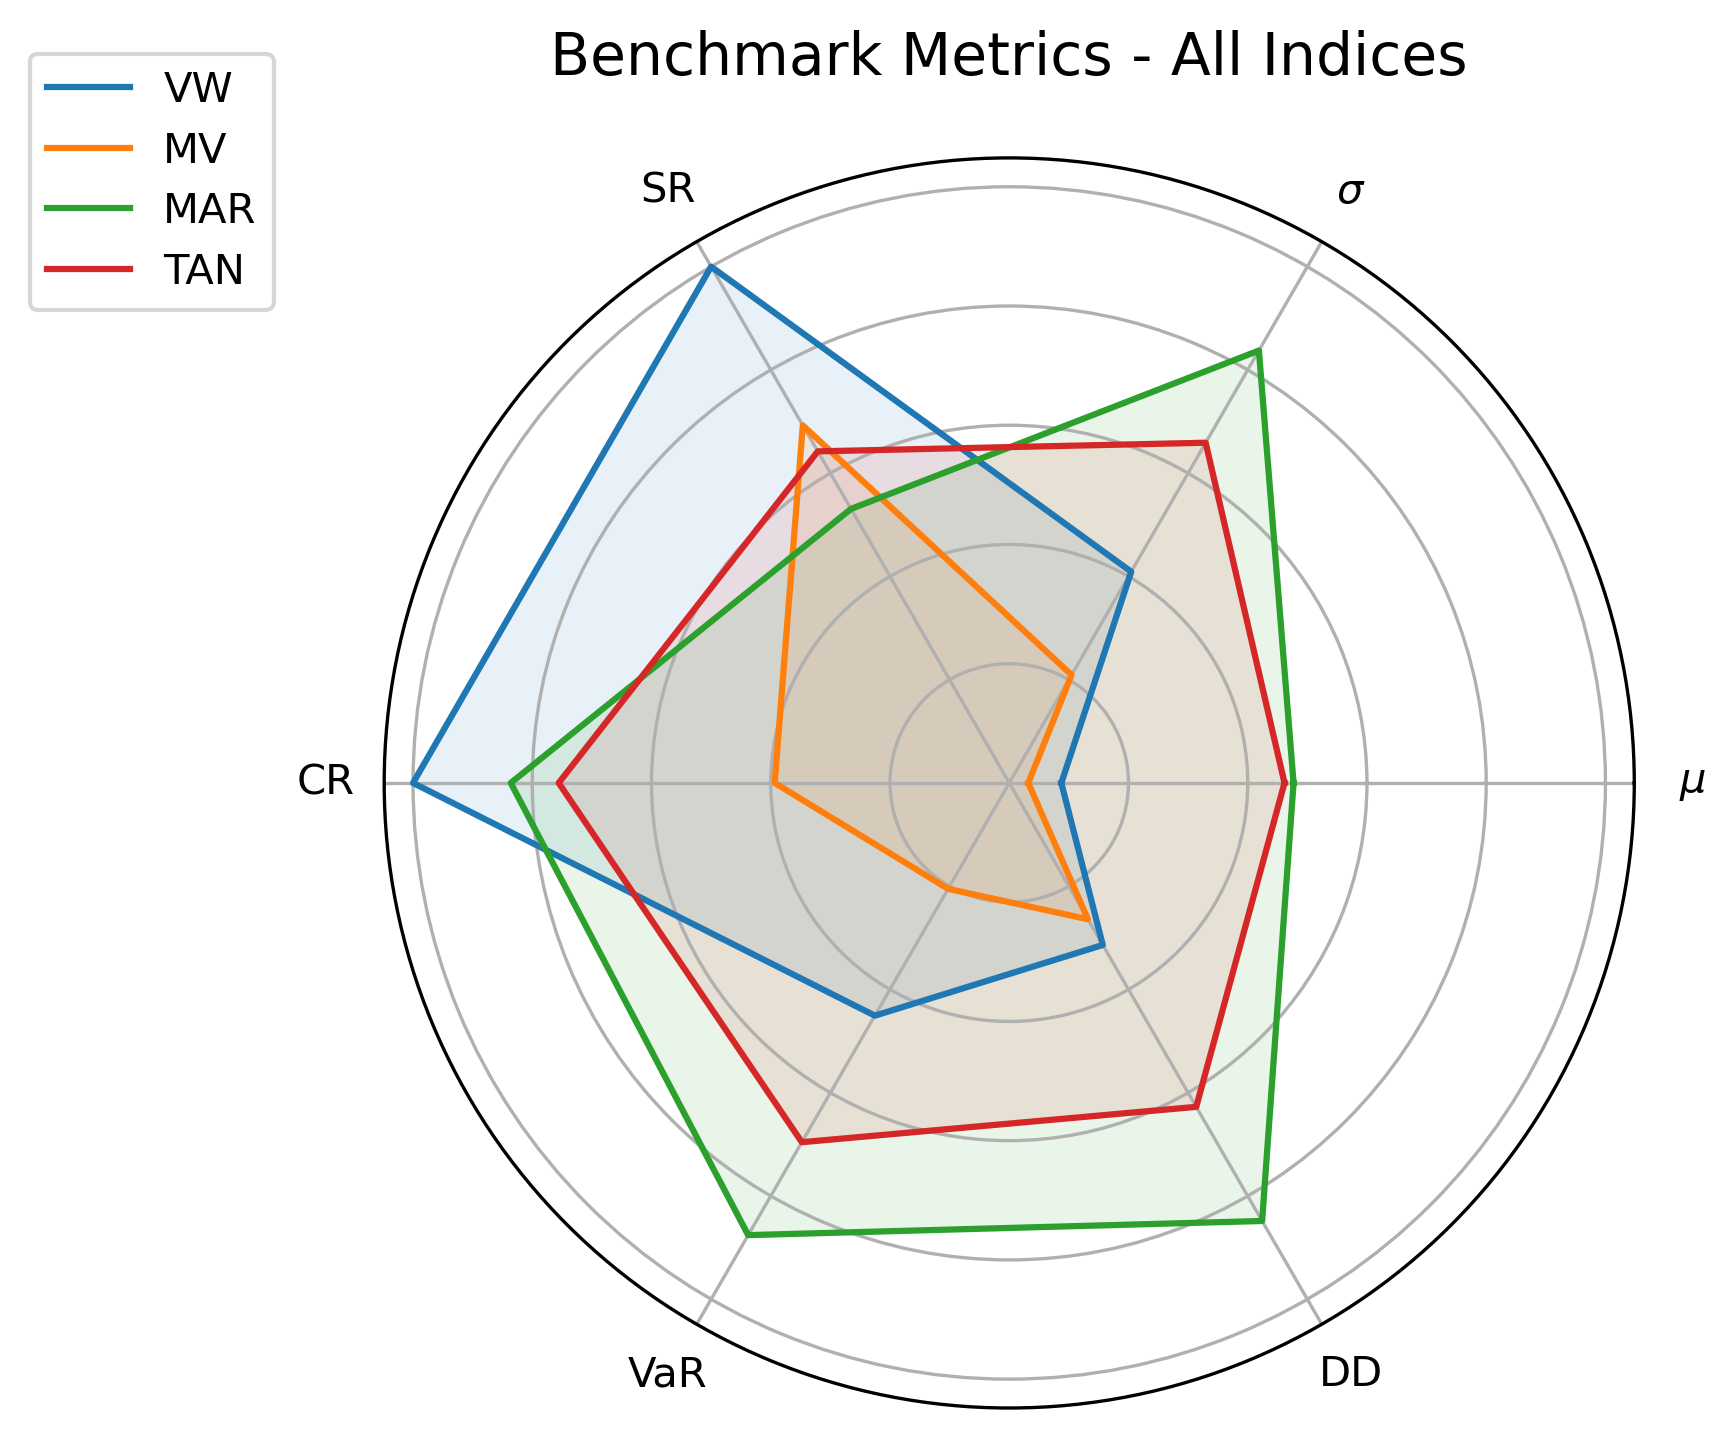
\includegraphics[width=\textwidth]{images/40_1.png}
\end{minipage}
\hfill
\begin{minipage}{0.48\textwidth}
  \centering
  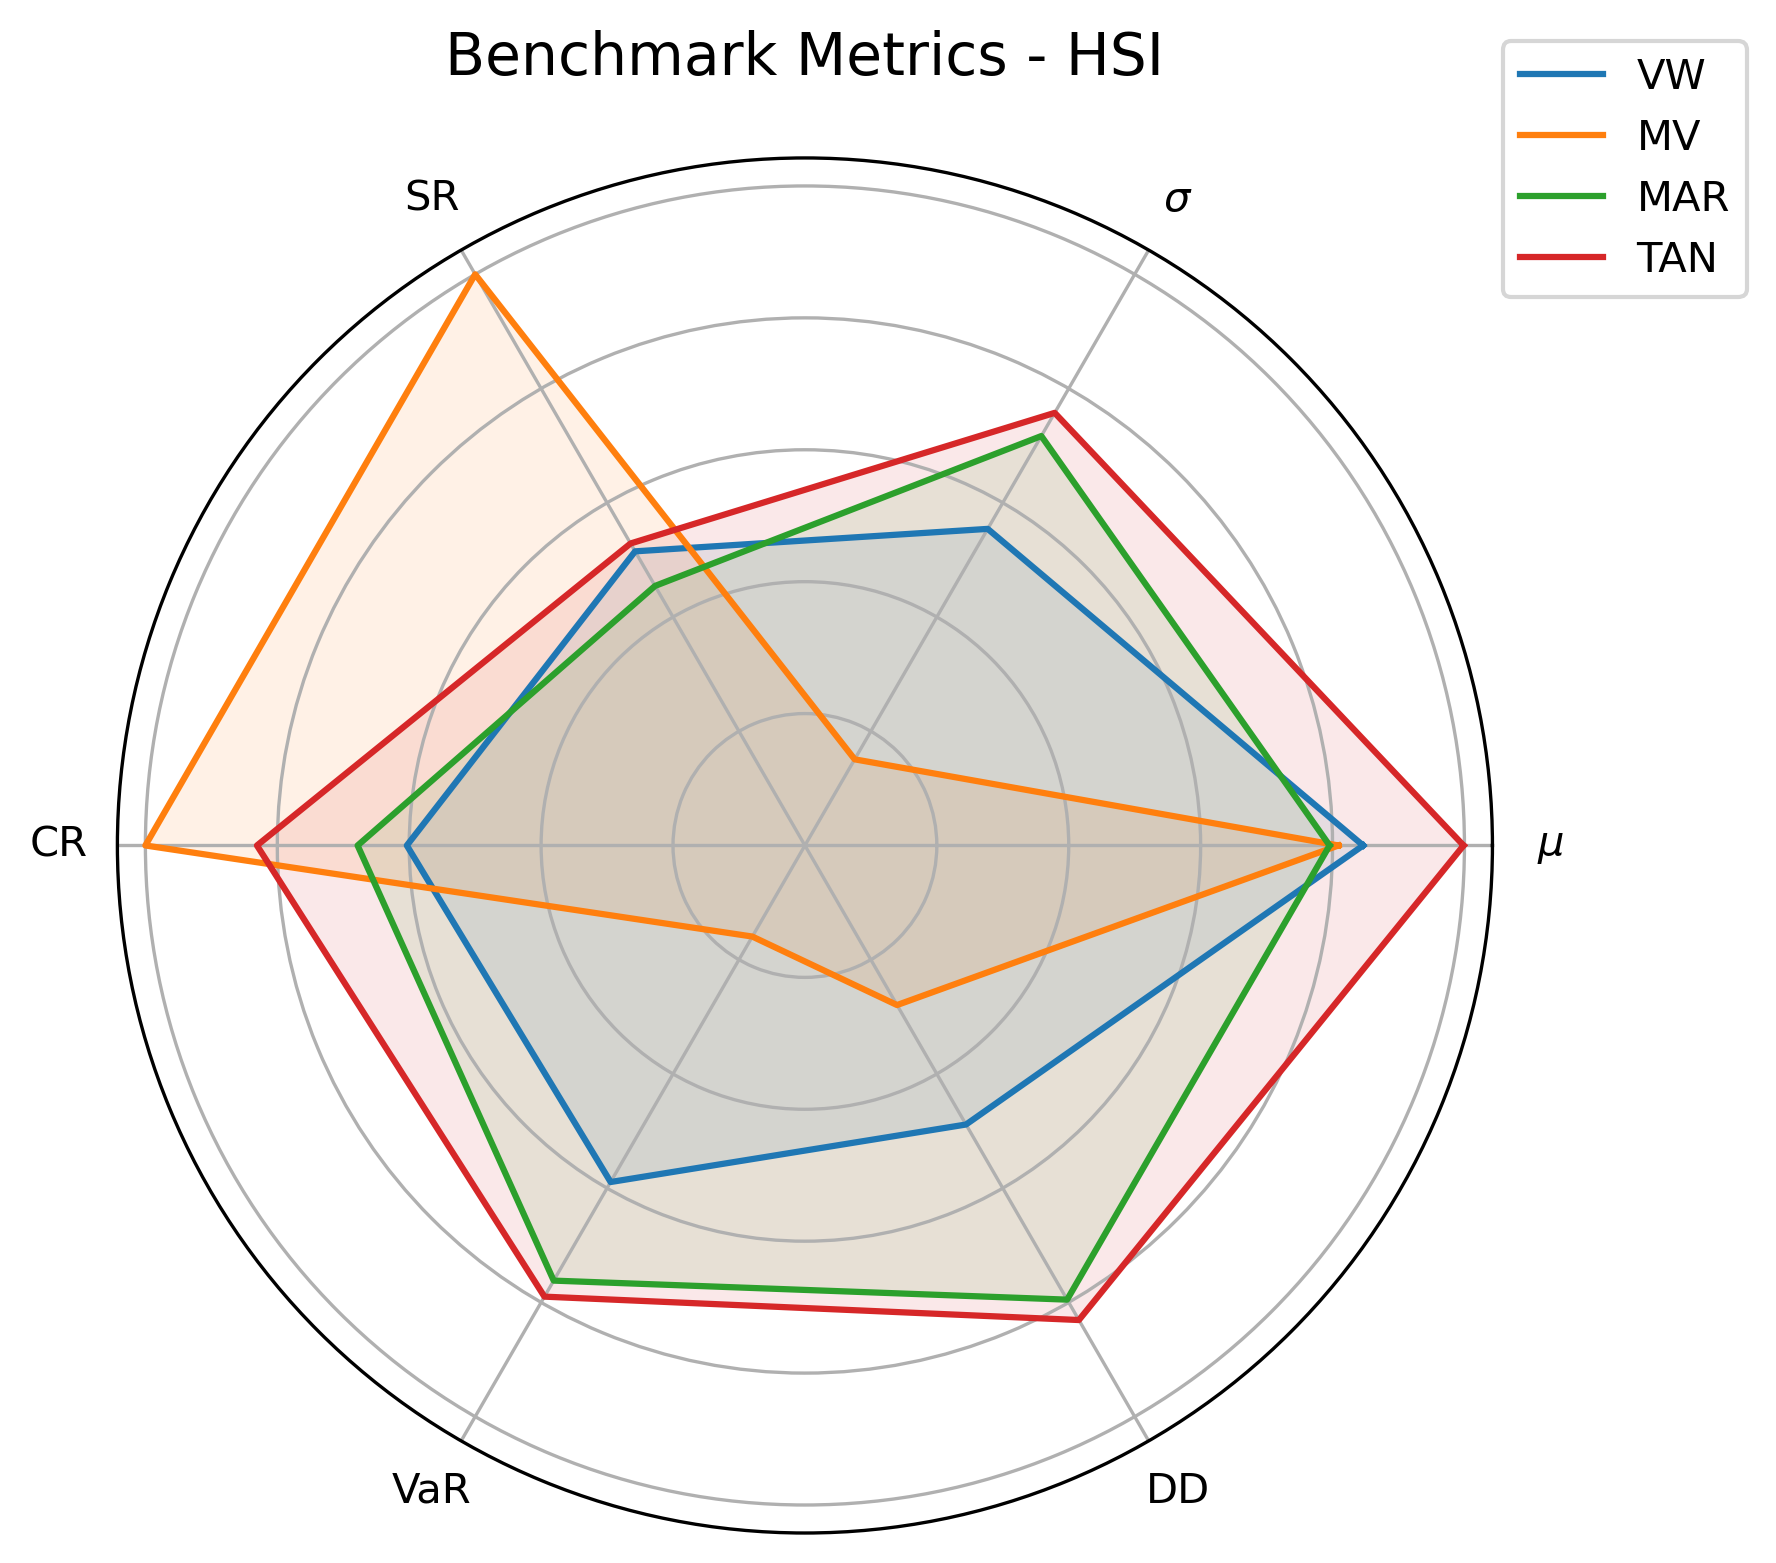
\includegraphics[width=\textwidth]{images/40_2.png}
\end{minipage}
\caption[Benchmark performance - Radar]{Performance comparison of benchmark portfolios (VW (blue); MV (orange); MAR (green) and TAN (red)) across six metrics: annualized return ($\mu$), volatility ($\sigma$), Sharpe ratio (SR), cumulative return (CR), 95\% VaR, and maximum drawdown (DD). All axes are scaled so that a larger radius indicates better performance; "bad" metrics ($\sigma$, VaR, DD) have been inverted.}
\label{fig:combined2}
\end{center}
\end{figure}

From these, we make several observations:
\begin{itemize}
\item The VW portfolios consistently offered the best trade-off between cumulative returns and the Sharpe Ratio. VW portfolios achieved the highest overall $SR$ in all indices except the HSI.
\item The MV portfolios offered the lowest $\sigma$ and $VaR$ across the board. Although MV did not record the lowest $DD$ in every index, a significant comparative improvement in drawdowns relative to other portfolios in the HSI index ensured that MV had the lowest $DD$ on average.
\item The MAR and TAN portfolios delivered the highest returns, but at the cost of high volatility, elevated $VaR$, and long drawdowns. Their risk profiles were so unfavorable that they ended up with lower ex-post Sharpe Ratios than the MV portfolio.
\end{itemize}
  
Due to the distinct behavior of the HSI index, where the usual performance patterns across benchmarks broke down, we include a separate radar plot focusing exclusively on HSI. Unlike the other indices, HSI saw the MV portfolio dominate across all metrics except $\mu$. The VW portfolio, typically one of the better performers, also struggled in HSI. While it still outperformed most return-optimized strategies in terms of $SR$ and $DD$, its advantage in cumulative return diminished. This contrast attests to the importance of evaluating portfolio performance across multiple indices, as each market may emphasize different strengths and weaknesses in a given strategy. Optimal strategy configurations will be discussed in detail in Section \ref{sec:localoptima}

\subsection{Standard GMM and KDE Results}
On average, the KDE portfolio behaved like a slightly riskier version of MV, achieving a modestly higher cumulative return at the cost of increased volatility. More notably, KDE outperformed MAR, its direct mean-variance counterpart, across all risk-focused metrics. It delivered a higher average Sharpe Ratio, lower volatility, and lower $VaR$, making it a meaningful improvement over the traditional approach. That said, KDE still lagged behind the value-weighted portfolio in terms of $CR$ and $SR$, despite offering a slight decrease in $\sigma$ and $VaR$.
\vspace{5mm}
\begin{table}[H]
  \centering
  \begin{tabular}{l*{7}{S[table-format=1.4]}}
  \toprule
  & {$\mu$} & {$\sigma$} & {SR} & {CR} & {VaR} & {DD} & {\textbar DD\textbar} \\
  \midrule
  VW & 0.0982 & 0.1814 & {\bfseries 0.4370} & {\bfseries 1.3317} & 0.2687 & 0.3534 & {\bfseries 3.0056} \\
  MV & 0.0849 & {\bfseries 0.1669} & 0.3895 & 1.0771 & {\bfseries 0.2423} & {\bfseries 0.3475} & 3.4809 \\
  MAR & {\bfseries 0.1922} & 0.2125 & 0.3645 & 1.2629 & 0.3143 & 0.4174 & 4.0214 \\
  KDE & 0.0853 & 0.1726 & 0.3801 & 1.0827 & 0.2529 & 0.3491 & 3.5437 \\
  GMM & 0.1737 & 0.2059 & 0.3107 & 1.0032 & 0.2986 & 0.4125 & 4.3024 \\
  \bottomrule
\end{tabular}

  \caption[Benchmark vs. KDE/GMM performance]{Annualized performance of benchmark, KDE, and GMM portfolios (Jan 2015-Mar 2025), averaged across all indices. Same metrics as in Table \ref{tab:single1}.}
  \label{tab:single2}
\end{table}

\begin{figure}[H]
\begin{center}
\begin{minipage}{1\textwidth}
  \centering
  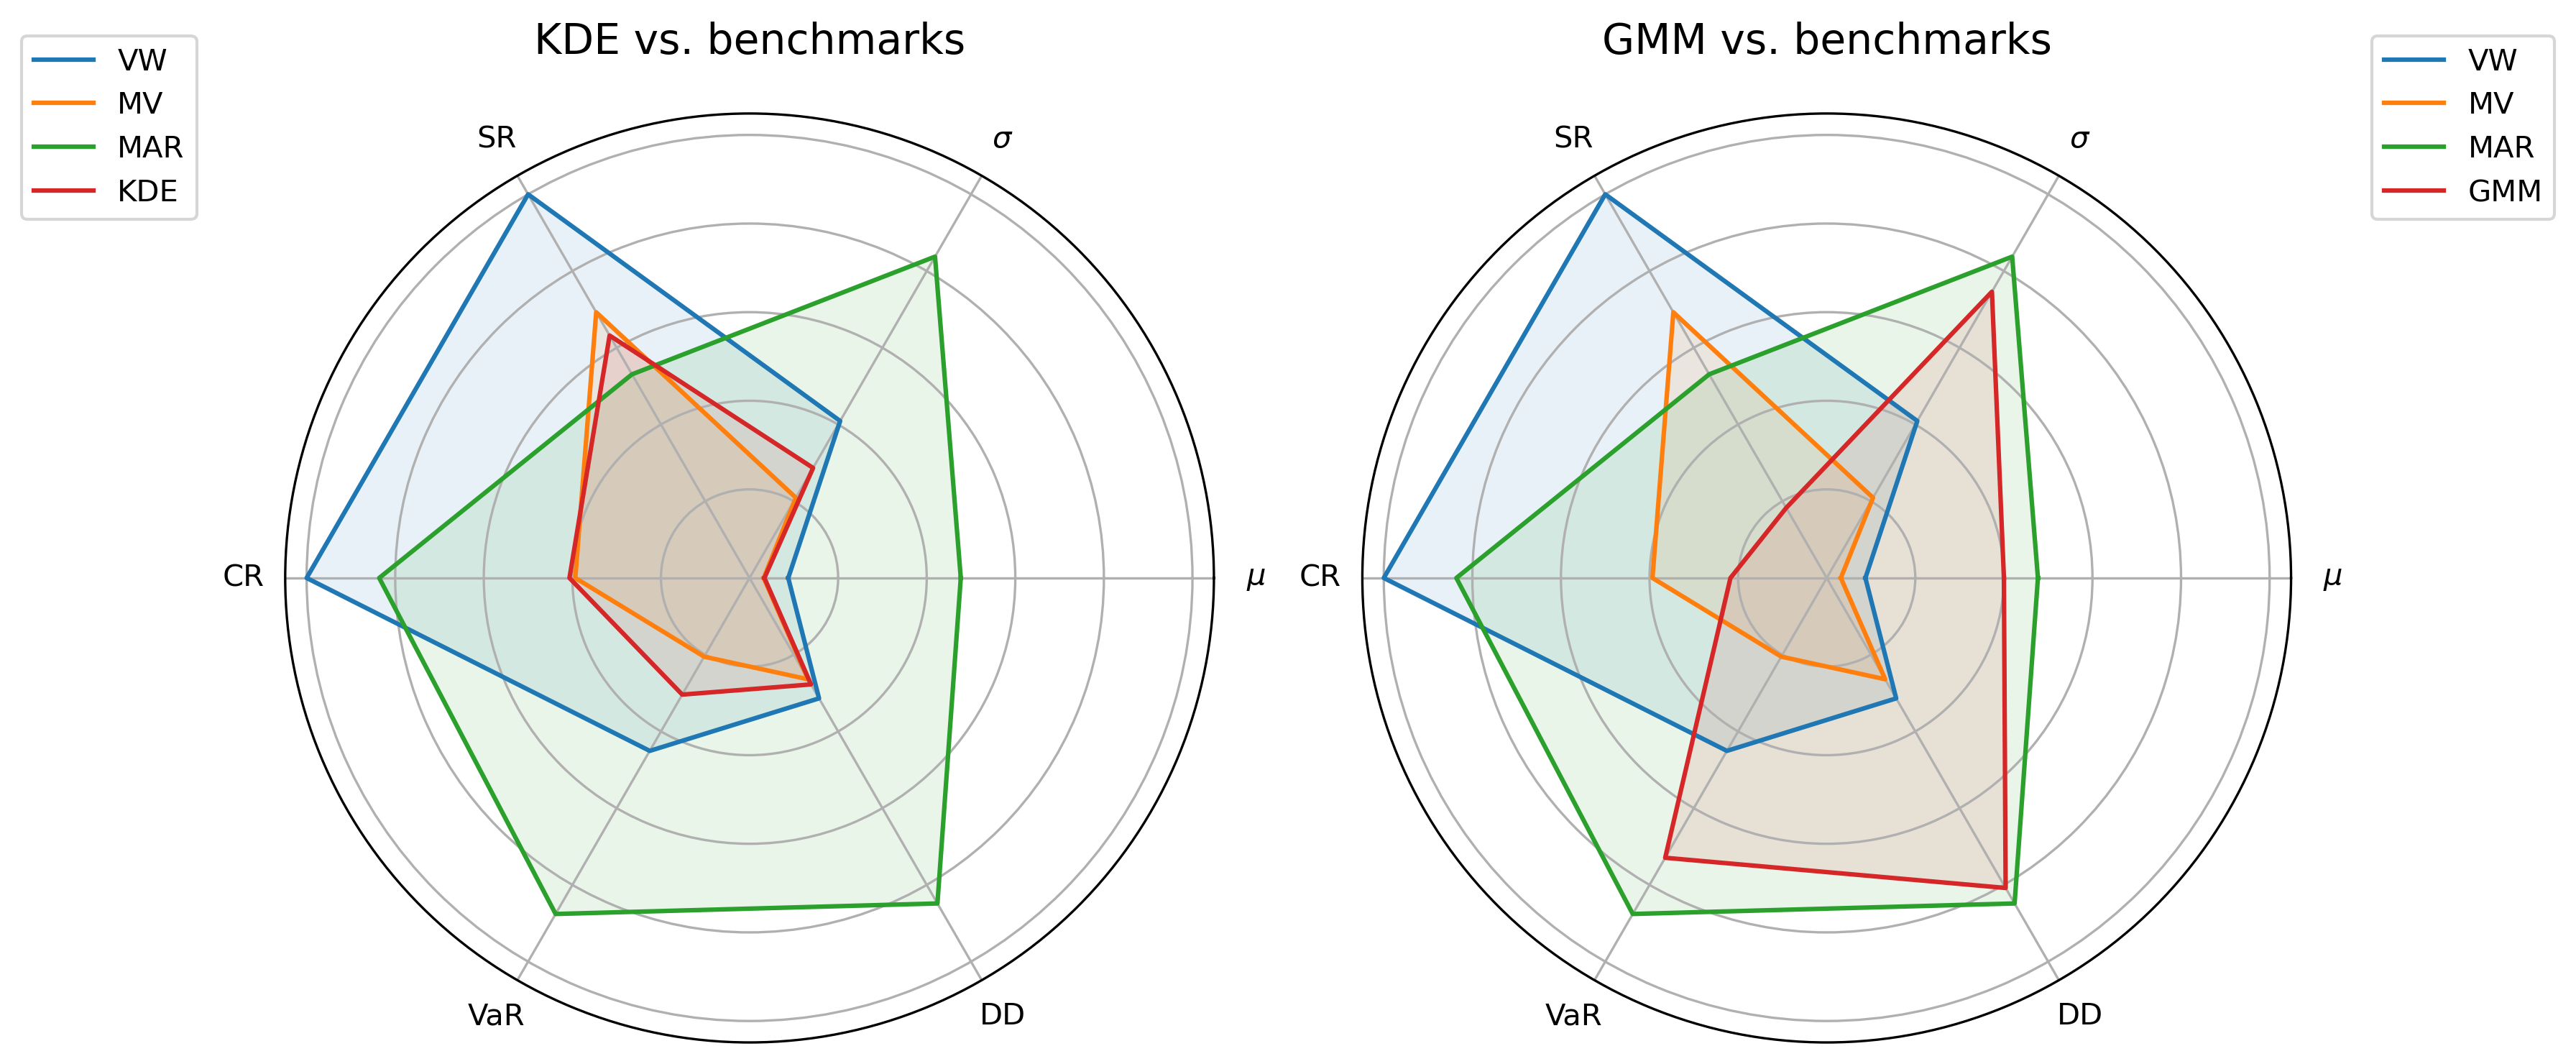
\includegraphics[width=\textwidth]{images/40_3.png}
\end{minipage}
\caption[Benchmark vs. KDE/GMM performance - Radar]{Radar-plot comparison of KDE (red, left) and GMM (red, right) portfolios against benchmark strategies VW (blue), MV (orange), and MAR (green). Same axes as in Figure \ref{fig:combined2}. The left panel shows the KDE portfolio, while the right panel shows the GMM portfolio.}
\label{fig:combined3}
\end{center}
\end{figure}

The GMM portfolio exhibited a return profile similar to that of MAR, but with noticeably worse risk-adjusted performance. While GMM improved slightly on all risk metrics compared to MAR, it still delivered the lowest cumulative return among all strategies, lower than that of the minimum-variance portfolio. As a result, its Sharpe Ratio was significantly lower than all other portfolios. Compared to the value-weighted, MV, and KDE portfolios, GMM's performance was disappointing. While it did achieve higher mean returns, it fell behind in every other metric and delivered an unattractive risk-return profile.

While the VW portfolio appears to dominate in this comparison, it is too early to draw definitive conclusions about the effectiveness of the KDE and GMM methods. The VW portfolio benefits from using the same information across all configurations, whereas KDE and GMM are sensitive to the data available within each setting. Hence, the averaged results presented here include many configurations with minimal data, making reliable estimation challenging for these density-based approaches. From Section \ref{sec:portability} onwards, we explore performance across different configurations and highlight the conditions under which these methods perform comparatively well.


\subsection{Tangency Portfolios}
\begin{table}[H]
  \centering
  \begin{tabular}{l*{7}{S[table-format=1.4]}}
  \toprule
  & {$\mu$} & {$\sigma$} & {SR} & {CR} & {VaR} & {DD} & {\textbar DD\textbar} \\
  \midrule
  VW & 0.0982 & 0.1814 & {\bfseries 0.4370} & {\bfseries 1.3317} & 0.2687 & 0.3534 & {\bfseries 3.0056} \\
  MV & 0.0849 & {\bfseries 0.1669} & 0.3895 & 1.0771 & {\bfseries 0.2423} & {\bfseries 0.3475} & 3.4809 \\
  TAN & 0.1885 & 0.1996 & 0.3817 & 1.2292 & 0.2950 & 0.3909 & 3.6075 \\
  TAN(KDE) & 0.1891 & 0.1939 & 0.3969 & 1.2379 & 0.2867 & 0.3793 & 3.4441 \\
  TAN(GMM) & {\bfseries 0.3184} & 0.2243 & 0.3266 & 1.0915 & 0.3277 & 0.4355 & 4.2121 \\
  \bottomrule
\end{tabular}

  \caption[Benchmark vs. TAN(KDE)/TAN(GMM) performance]{Annualized performance of benchmark, TAN(KDE), and TAN(GMM) portfolios (Jan 2015-Mar 2025), averaged across all indices. Same metrics as in Table \ref{tab:single1}.}
  \label{tab:single3}
\end{table}

\vspace{5mm}
\begin{figure}[H]
\begin{center}
\begin{minipage}{1\textwidth}
  \centering
  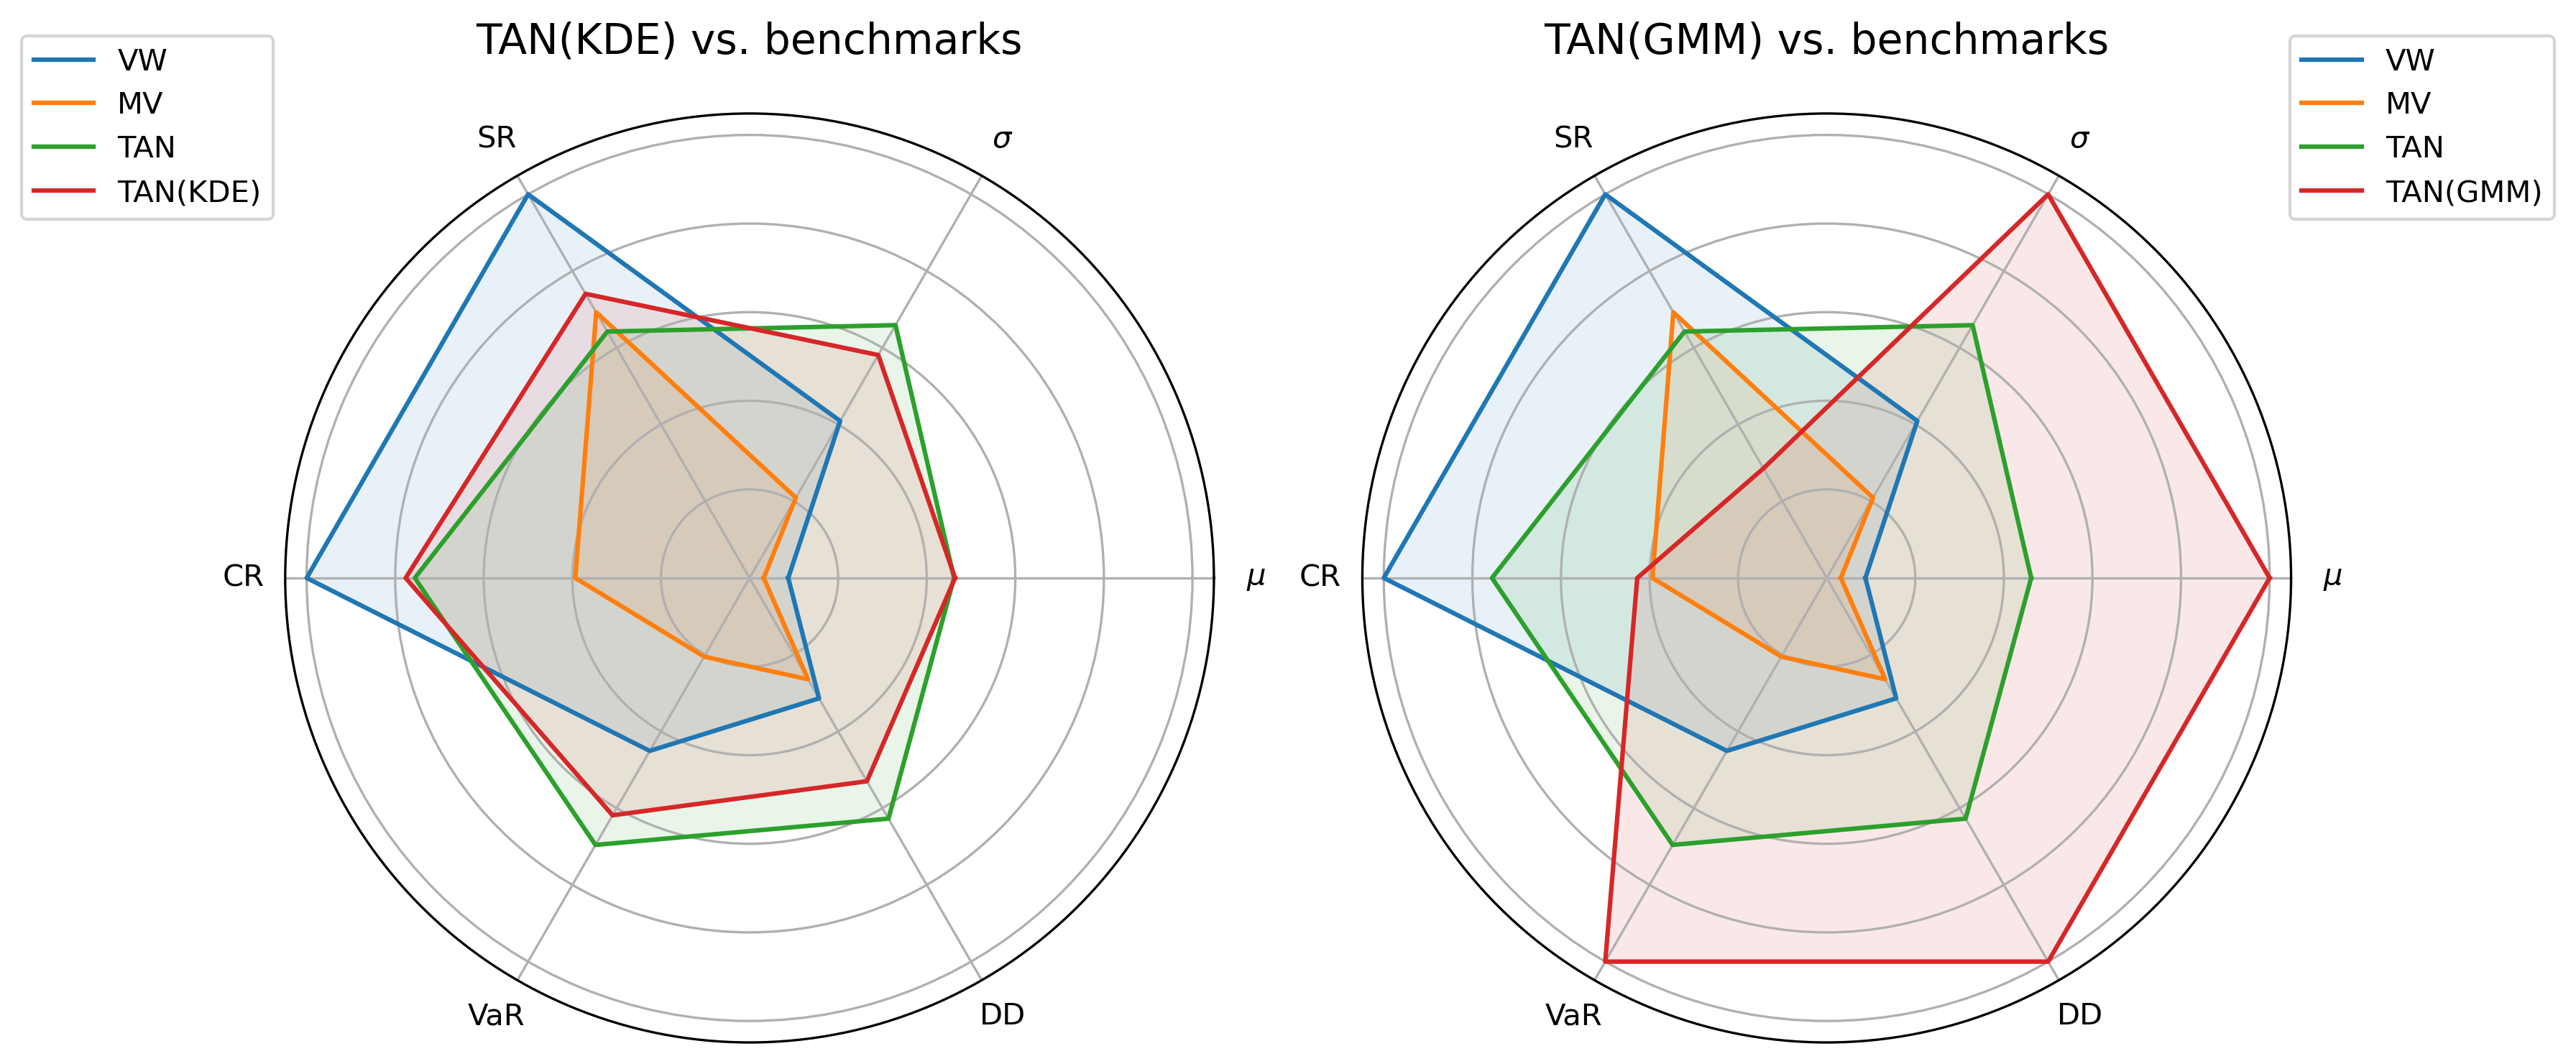
\includegraphics[width=\textwidth]{images/40_4.png}
\end{minipage}
\caption[Benchmark vs. TAN(KDE)/TAN(GMM) performance - Radar]{Radar-plot comparison of TAN(KDE) (red, left) and TAN(GMM) (red, right) portfolios against benchmark strategies VW (blue), MV (orange), and MAR (green). Same axes as in Figure \ref{fig:combined2}. The left panel shows the TAN(KDE) portfolio, while the right panel shows the TAN(GMM) portfolio.}
\label{fig:combined4}
\end{center}
\end{figure}

The TAN(KDE) portfolio delivered strong overall results, achieving the second-highest average Sharpe Ratio across all portfolios. Compared to its direct counterpart, TAN, TAN(KDE) showed a slightly higher cumulative return and Sharpe Ratio, lower volatility, lower Value-at-Risk, and smaller drawdowns. Notably, TAN(KDE) even outperformed the MV portfolio in terms of maximum drawdown within the S\&P500 index, which is surprising given how consistently MV tends to lead on downside risk measures. This performance is especially noteworthy because it emerges despite averaging across all configurations, including many highly data-sparse and inherently challenging for KDE-based estimation. This suggests that TAN(KDE) can deliver a favorable risk-return profile even under varying conditions.

The TAN(GMM) portfolio produced the most extreme results among all strategies. It achieved the highest average mean return, but also the highest volatility, $VaR$, and maximum drawdown. Its risk-adjusted performance was poor despite the strong headline return, with a Sharpe Ratio that fell below that of both TAN and TAN(KDE). Compared to TAN(KDE), it performed worse across every risk metric. In the end, TAN(GMM) managed to maximize not only returns, but also risk.


\section{Strategy Portability}
\label{sec:portability}

Next, we evaluate each portfolio strategy under its most favorable conditions. We define the "best" configuration as the parameter set (data frequency, lookback window, rebalancing interval, and investment universe size) that achieves the highest penalized Sharpe Ratio, averaged across all indices.

The penalized Sharpe Ratio ($SR_p$) balances high average returns against consistency in performance across multiple asset-selection seeds. For portfolio $k$, it is calculated as:
$$SR_{p,k} = \mathbb{E}[SR_k] - \lambda \cdot \sqrt{Var[SR_k]}$$
Or explicitly:
$$SR_{p,k} = \frac{1}{n} \sum_{i=1}^{n} SR_{k,i} - \lambda \cdot \sqrt{ \frac{1}{n} \sum_{i=1}^{n} \left( SR_{k,i} - \frac{1}{n} \sum_{i=1}^{n} SR_{k,i} \right)^2 }$$
Here, $SR_{k,i}$ represents the Sharpe Ratio obtained with seed $i$, and the parameter $\lambda$ controls the penalty imposed for variability across seeds. We use $\lambda=1$, making the penalized Sharpe Ratio the mean Sharpe Ratio minus its standard deviation.

In this Section, we select a single optimal configuration per strategy based on the highest average penalized Sharpe Ratio across all four indices. Identifying a globally effective parameter set and testing it locally allows us to determine how well the strategies generalize. The table below summarizes these optimal configurations ranked by their penalized Sharpe Ratios. Section \ref{sec:localoptima} will discuss index-specific optimal configurations.

\begin{table}[H]
  \centering
  \begin{tabular}{l*{5}{S[table-format=1.4]}}
  \toprule
  & {Reb.} & {Wnd.(mo)} & {Data} & {SR} & {SR$_p$} \\
  \midrule
  VW & {annual} & {5years} & {monthly} & 0.4835 & {\bfseries 0.3788} \\
  MV & {monthly} & {3months} & {daily} & {\bfseries 0.5005} & 0.3773 \\
  KDE & {monthly} & {6months} & {daily} & 0.4714 & 0.3587 \\
  TAN(KDE) & {monthly} & {5years} & {monthly} & 0.4812 & 0.3467 \\
  MAR & {annual} & {1years} & {daily} & 0.4599 & 0.3251 \\
  TAN & {monthly} & {5years} & {monthly} & 0.4624 & 0.3094 \\
  TAN(GMM) & {annual} & {5years} & {monthly} & 0.4071 & 0.2330 \\
  GMM & {monthly} & {1years} & {weekly} & 0.3627 & 0.1947 \\
  \bottomrule
\end{tabular}

  \caption[Best configurations - Global]{Optimal parameter settings per strategy, ranked by average penalized Sharpe ratio across all four indices and portfolio sizes. Columns report rebalancing frequency (Reb.), lookback window in months (Wnd.), data frequency (Data), annualized Sharpe ratio (SR), and penalized Sharpe ratio ($SR_p$). Boldface highlights the best value in each column.}
  \label{tab:single4}
\end{table}

Table \ref{tab:single4} presents the MV portfolio achieving the highest raw Sharpe ratio, while the VW strategy claims the top penalized Sharpe ratio, which demonstrates their superior consistency across different markets. The KDE-based portfolios follow closely, with both vanilla KDE and TAN(KDE) delivering strong risk-adjusted performance. The tangency portfolio using KDE ranks third in Sharpe ratio while posting an average penalized Sharpe ratio. In contrast, the GMM portfolios show weaker performance overall, with both GMM and TAN(GMM) achieving the lowest penalized and raw Sharpe ratios, reflecting high dispersion across configurations.

Having identified the best configuration for each strategy based on global performance, we now evaluate how well these configurations carry over across individual indices.

\begin{center}
  \textbf{FTSE100}
\end{center}
\begin{table}[H]
  \centering
  \begin{tabular}{l*{7}{S[table-format=1.4]}}
  \toprule
  & {$\mu$} & {$\sigma$} & {CR} & {SR} & {VaR} & {DD} & {\textbar DD\textbar} \\
  \midrule
  VW & 0.0736 & 0.1199 & 0.9246 & 0.4455 & 0.1675 & 0.2439 & 1.5833 \\
  MV & 0.0675 & {\bfseries 0.1101} & 0.8185 & 0.4371 & {\bfseries 0.1673} & {\bfseries 0.1914} & {\bfseries 1.2077} \\
  MAR & 0.0768 & 0.2199 & 0.6530 & 0.2602 & 0.3350 & 0.5552 & 6.1615 \\
  TAN & 0.0379 & 0.1404 & 0.3231 & 0.1197 & 0.1921 & 0.3003 & 3.5833 \\
  KDE & 0.1070 & 0.1265 & 1.5705 & {\bfseries 0.6865} & 0.1829 & 0.2826 & 1.2385 \\
  GMM & {\bfseries 0.1171} & 0.1804 & {\bfseries 1.6224} & 0.5432 & 0.2380 & 0.3034 & 2.9423 \\
  TAN(KDE) & 0.0578 & 0.1335 & 0.6241 & 0.2761 & 0.2020 & 0.2767 & 3.4167 \\
  TAN(GMM) & 0.0624 & 0.1648 & 0.6189 & 0.2339 & 0.2734 & 0.3568 & 3.5833 \\
  \bottomrule
\end{tabular}

  \caption[Global best configuration - All strategies - FTSE100]{Annualized performance of all portfolios (Jan 2015-Mar 2025), FTSE100 only. Averaged across all portfolio sizes. Same metrics as in Table \ref{tab:single1}.}
  \label{tab:single5}
\end{table}

In the FTSE100, the MV portfolio significantly outperformed all other strategies in terms of risk management, though its $VaR$ uplift over VW, the second safest portfolio, was marginal. Despite its strong risk metrics, MV did not reach the highest Sharpe Ratio, as its returns remained modest.

\vspace{5mm}
\begin{figure}[H]
  \begin{center}
  \begin{minipage}{1\textwidth}
    \centering
    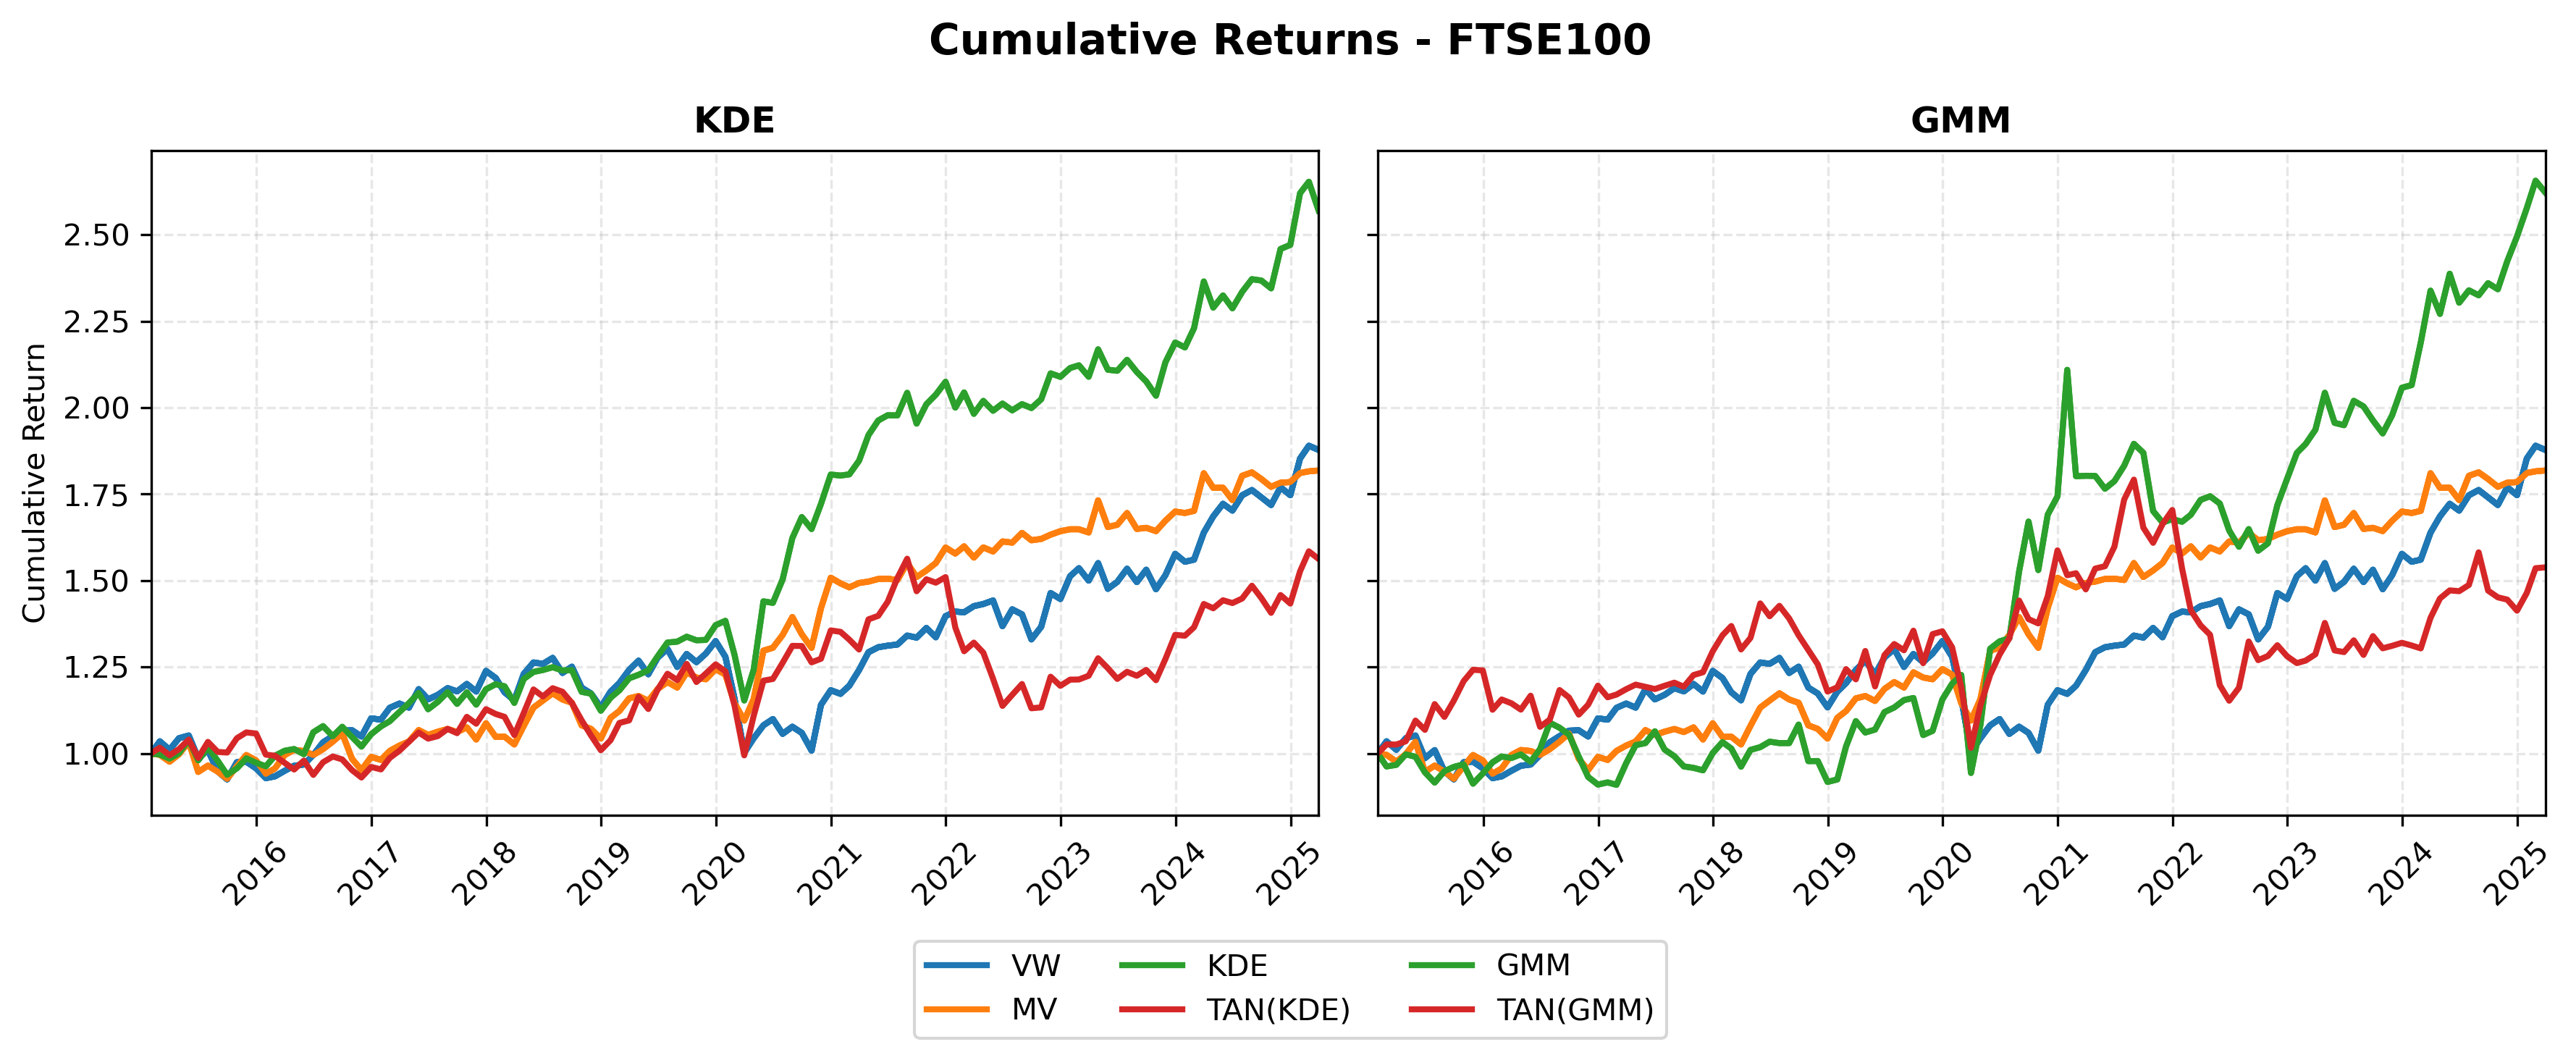
\includegraphics[width=\textwidth]{images/40_6.png}
  \end{minipage}
  \caption[Global best configuration - FTSE100 - Cumulative returns]{Cumulative returns (Jan 2015-Mar 2025) of the best global configuration per strategy on the FTSE100 index. Left panel: default KDE (green) and its tangency variant TAN(KDE) (red) versus benchmarks VW (blue) and MV (orange). Right panel: default GMM (green) and its tangency variant TAN(GMM) (red) versus the same benchmarks. All series are indexed to 1.0 at the start date.}
  \label{fig:combined6}
  \end{center}
  \end{figure}

The KDE portfolio achieved a higher cumulative return than VW and MV, allowing it to outperform them and take the lead in terms of the Sharpe Ratio. However, this came at the cost of worse risk metrics. In contrast, the TAN(KDE) portfolio offered subpar risk metrics and cumulative return. Nevertheless, it had the highest $SR$ among the tangency portfolios, which all performed surprisingly unwell in the FTSE100.

GMM delivers the highest average returns but comes with elevated volatility and $VaR$ that exceed most other strategies. The TAN(GMM) portfolio follows the pattern of tangency underperformance, with substantially lower returns and higher risk metrics than GMM.

% \newpage
\begin{center}
  \textbf{HSI}
\end{center}
In the HSI index, the MV portfolio achieved top-of-the-line performance across the board, leading in all metrics besides mean return and drawdown duration. Surprisingly, the VW portfolio performed poorly, showing the lowest Sharpe Ratio and one of the lowest cumulative returns. This comparative underperformance of VW is unique to the HSI index.

\begin{table}[H]
  \centering
  \begin{tabular}{l*{7}{S[table-format=1.4]}}
  \toprule
  & {$\mu$} & {$\sigma$} & {CR} & {SR} & {VaR} & {DD} & {\textbar DD\textbar} \\
  \midrule
  VW & 0.0593 & 0.2141 & 0.4375 & 0.1391 & 0.3292 & 0.5080 & 4.0833 \\
  MV & 0.0952 & {\bfseries 0.1340} & {\bfseries 1.2643} & {\bfseries 0.5613} & {\bfseries 0.2014} & {\bfseries 0.3036} & 4.8769 \\
  MAR & 0.1006 & 0.2391 & 0.9545 & 0.3366 & 0.3693 & 0.4551 & 6.2231 \\
  TAN & 0.0776 & 0.2191 & 0.6878 & 0.2324 & 0.3531 & 0.5864 & {\bfseries 3.7500} \\
  KDE & 0.0736 & 0.1376 & 0.8471 & 0.3923 & 0.2164 & 0.3791 & 4.7654 \\
  GMM & 0.0432 & 0.1698 & 0.3296 & 0.1380 & 0.2646 & 0.4636 & 6.9615 \\
  TAN(KDE) & 0.0613 & 0.2226 & 0.4317 & 0.1539 & 0.3851 & 0.5999 & {\bfseries 3.7500} \\
  TAN(GMM) & {\bfseries 0.1056} & 0.3890 & 0.4200 & 0.2031 & 0.4020 & 0.7050 & {\bfseries 3.7500} \\
  \bottomrule
\end{tabular}

  \caption[Global best configuration - All strategies - HSI]{Annualized performance of all portfolios (Jan 2015-Mar 2025), HSI only. Averaged across all portfolio sizes. Same metrics as in Table \ref{tab:single1}.}
  \label{tab:single6}
\end{table}

The KDE portfolio improved significantly over VW in both the Sharpe Ratio and cumulative return, while maintaining better downside risk metrics. However, the TAN(KDE) portfolio underperformed, with a lower cumulative return and unattractive risk metrics. This underperformance was shared between all tangency portfolios on the HSI.

\vspace{5mm}
\begin{figure}[H]
  \begin{center}
  \begin{minipage}{1\textwidth}
    \centering
    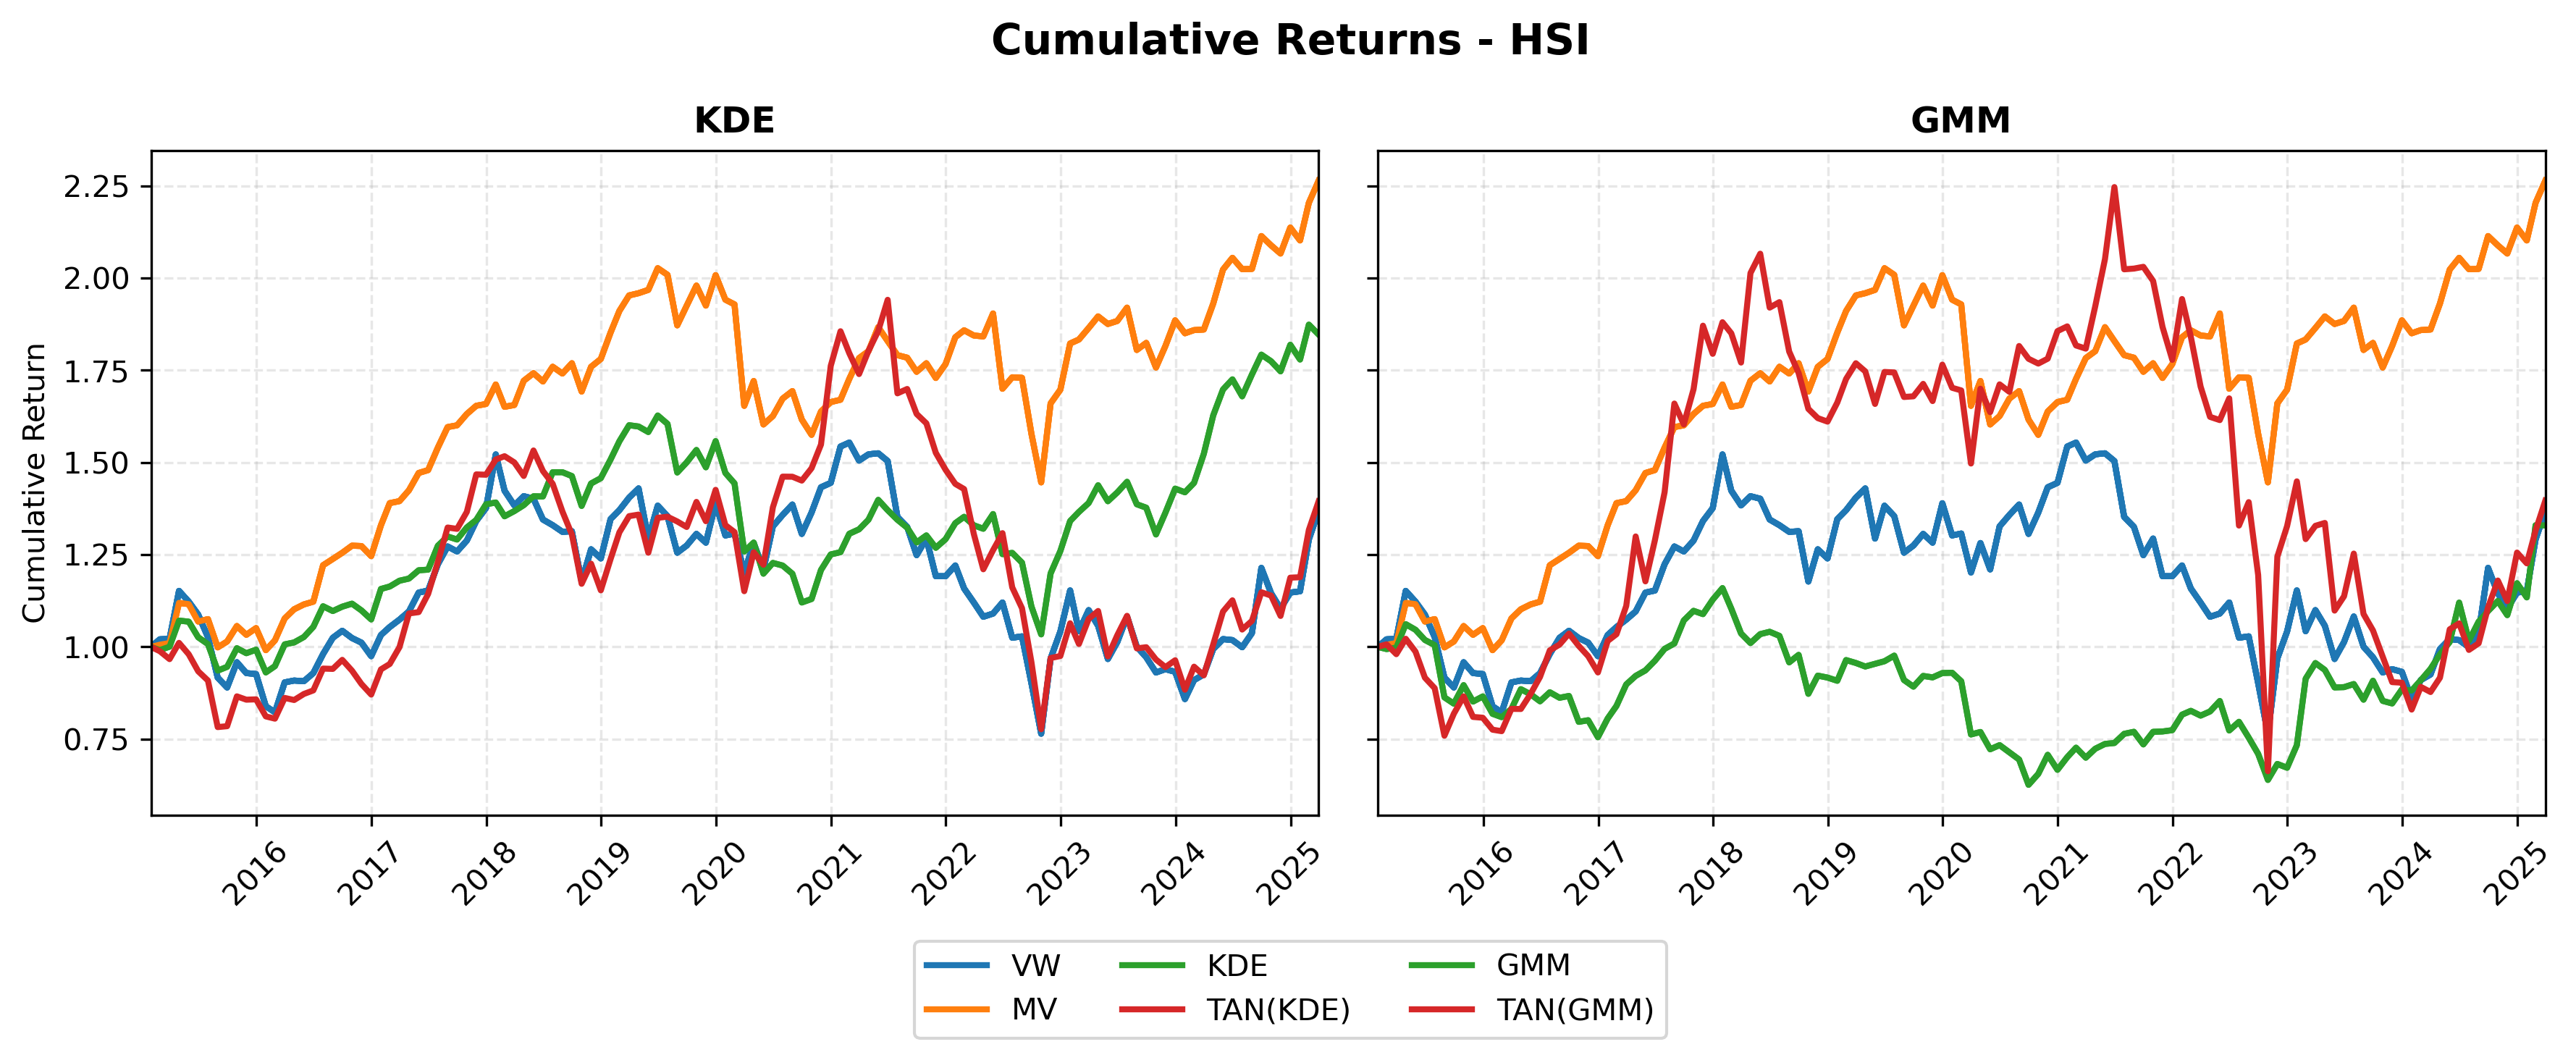
\includegraphics[width=\textwidth]{images/40_7.png}
  \end{minipage}
  \caption[Global best configuration - HSI - Cumulative returns]{Cumulative returns (Jan 2015-Mar 2025) of the best global configuration per strategy on the HSI index. Same layout as Figure \ref{fig:combined6}.}
  \label{fig:combined7}
  \end{center}
  \end{figure}

The GMM portfolio achieved decently low volatility, but at the cost of the lowest cumulative return. On the positive side, GMM did not suffer from the same cataclysmic drawdown of its tangency variant. The TAN(GMM) portfolio was the riskiest of all strategies, with the deepest downside.

\newpage
\begin{center}
  \textbf{S\&P500}
\end{center}
\begin{table}[H]
  \centering
  \begin{tabular}{l*{7}{S[table-format=1.4]}}
  \toprule
  & {$\mu$} & {$\sigma$} & {CR} & {SR} & {VaR} & {DD} & {\textbar DD\textbar} \\
  \midrule
  VW & 0.1373 & 0.1520 & 2.3288 & 0.8406 & 0.2313 & 0.2358 & 1.9167 \\
  MV & 0.0735 & {\bfseries 0.0953} & 0.9649 & 0.5650 & {\bfseries 0.1256} & 0.2380 & 1.8115 \\
  MAR & {\bfseries 0.2353} & 0.2505 & {\bfseries 5.2266} & {\bfseries 0.8490} & 0.3917 & 0.3695 & 2.2077 \\
  TAN & 0.1251 & 0.1591 & 1.9467 & 0.6802 & 0.2752 & 0.1986 & 1.8333 \\
  KDE & 0.0993 & 0.1205 & 1.4329 & 0.6573 & 0.1699 & 0.2484 & {\bfseries 1.7846} \\
  GMM & 0.0525 & 0.1964 & 0.3806 & 0.1754 & 0.2961 & 0.4608 & 6.1538 \\
  TAN(KDE) & 0.1236 & 0.1459 & 1.9678 & 0.7309 & 0.2351 & {\bfseries 0.1585} & 2.0833 \\
  TAN(GMM) & 0.1792 & 0.2021 & 3.4388 & 0.7928 & 0.2889 & 0.2532 & 2.0833 \\
  \bottomrule
\end{tabular}

  \caption[Global best configuration - All strategies - S\&P500]{Annualized performance of all portfolios (Jan 2015-Mar 2025), S\&P500 only. Averaged across all portfolio sizes. Same metrics as in Table \ref{tab:single1}.}
  \label{tab:single7}
\end{table}

\begin{figure}[H]
  \begin{center}
  \begin{minipage}{1\textwidth}
    \centering
    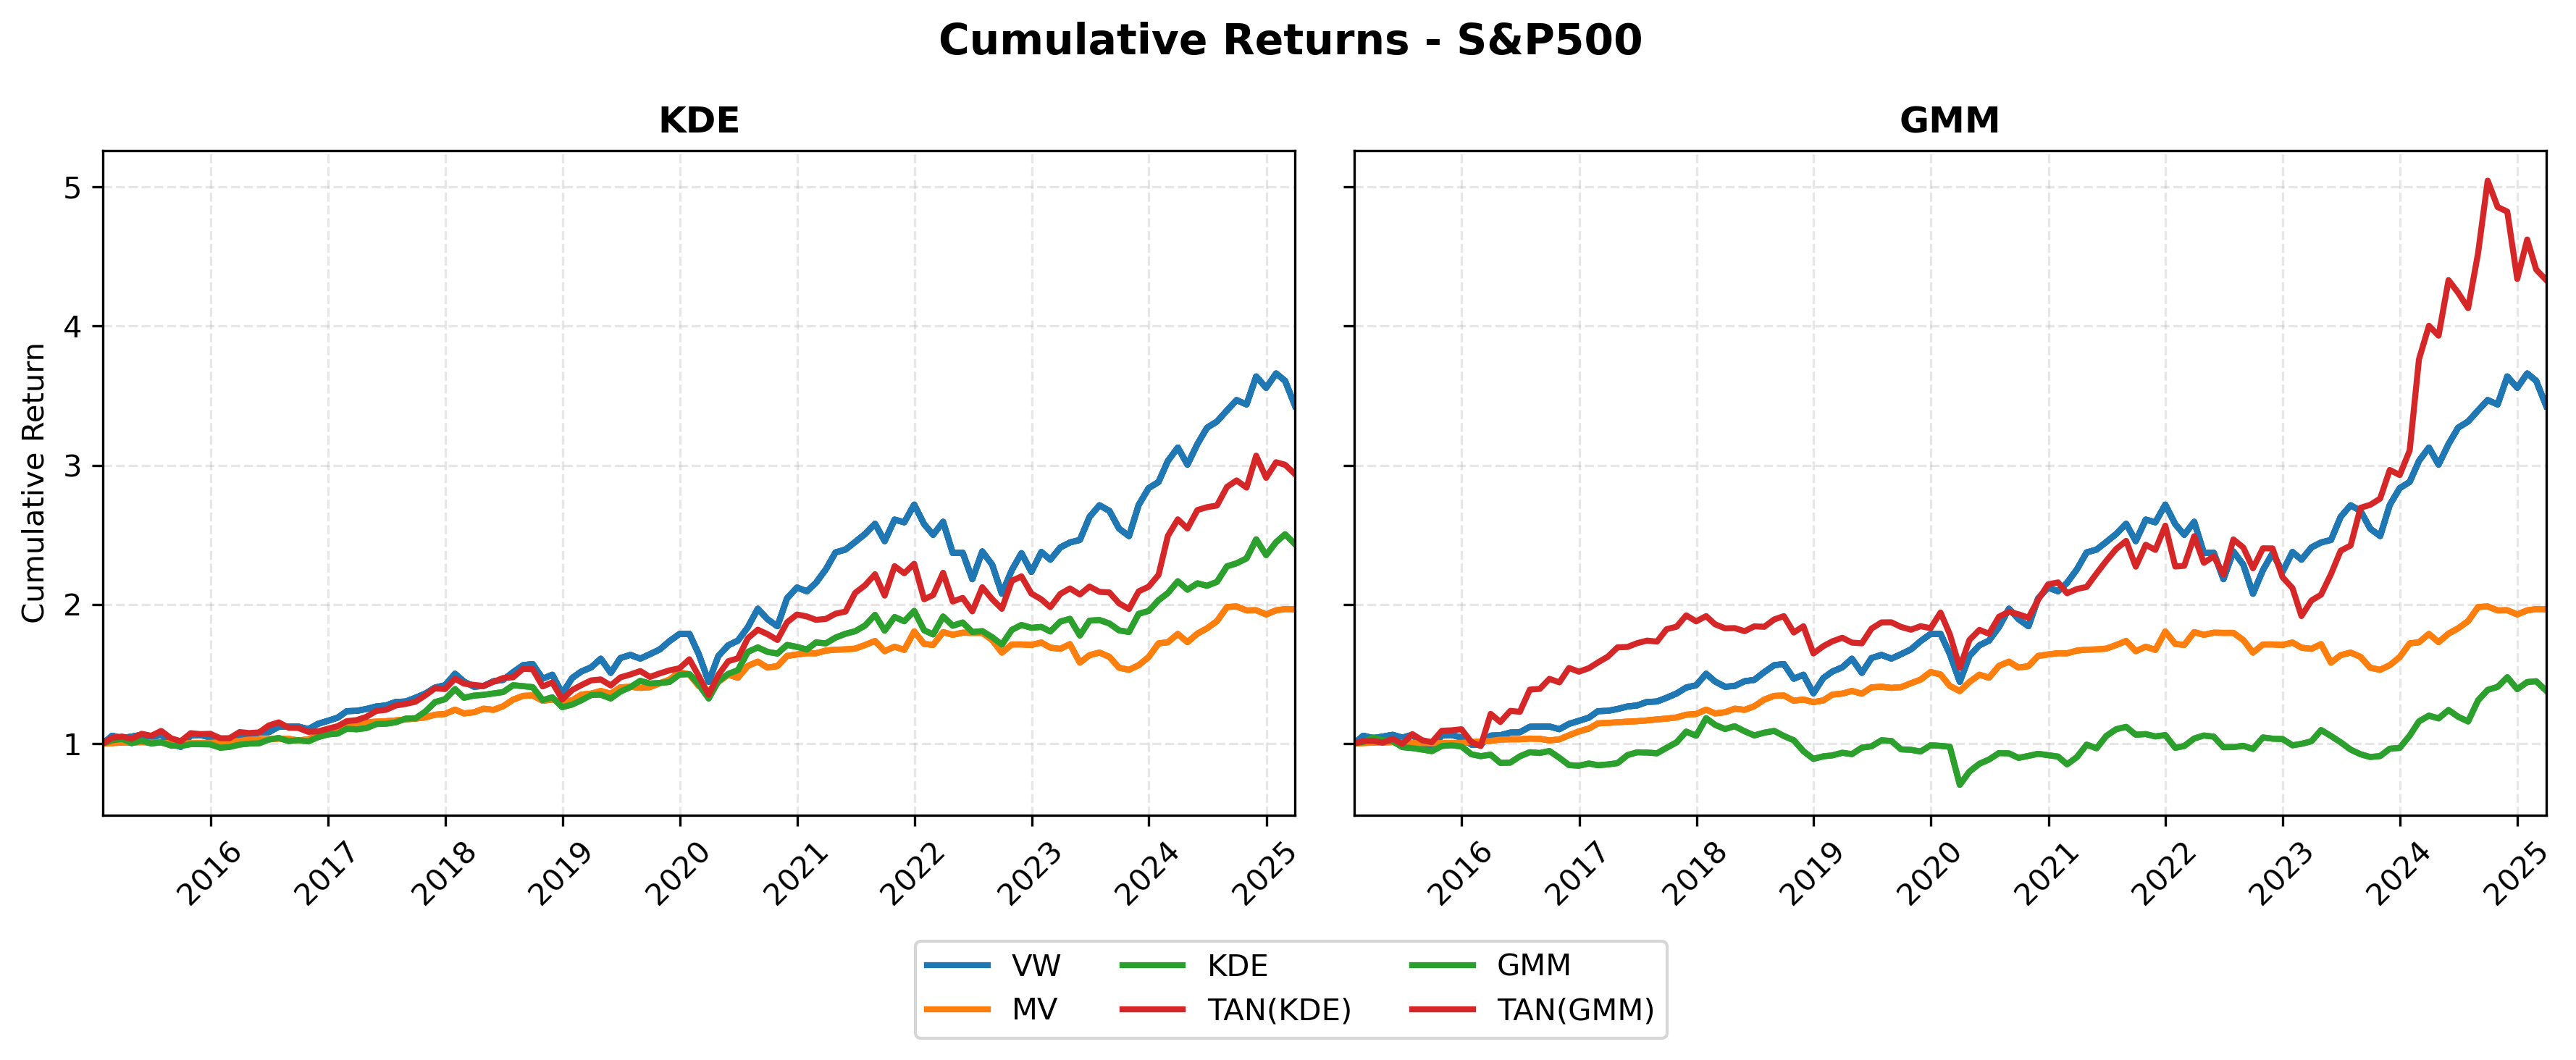
\includegraphics[width=\textwidth]{images/40_8.png}
  \end{minipage}
  \caption[Global best configuration - S\&P500 - Cumulative returns]{Cumulative returns (Jan 2015-Mar 2025) of the best global configuration per strategy on the S\&P500 index. Same layout as Figure \ref{fig:combined6}.}
  \label{fig:combined8}
  \end{center}
  \end{figure}

In the S\&P500, the VW portfolio delivered its best performance, with the second-best Sharpe Ratio and a competitive cumulative return. The MV portfolio again maintained the lowest volatility and $VaR$, although it did not lead in terms of drawdown length or depth.

The KDE portfolio performed modestly on most metrics, underdelivering in return and risk-adjusted terms. Its relative strength was in $|DD|$ and $VaR$, where it achieved the best and second-best results, respectively. In contrast, TAN(KDE) ranked among the best performers in cumulative return while offering a strong risk profile, including the shallowest drawdown of any portfolio in the S\&P, 7.9\% lower than the MV strategy.

The GMM portfolio proved to be the weakest performer in the S\&P500. It delivered the lowest cumulative return and Sharpe ratio of any strategy, while also suffering the highest volatility, worst VaR, and deepest drawdown. Its reliance on just six months of monthly data for nearly 500 assets likely exacerbates its instability, a point we revisit in Section \ref{sec:localoptima}. By comparison, the TAN(GMM) delivered a more moderate risk profile. Though its returns, volatility, and drawdown fail to entice when compared to other strategies.

\begin{center}
  \textbf{STOXX50}
\end{center}
\begin{table}[H]
  \centering
  \begin{tabular}{l*{7}{S[table-format=1.4]}}
  \toprule
  & {$\mu$} & {$\sigma$} & {CR} & {SR} & {VaR} & {DD} & {\textbar DD\textbar} \\
  \midrule
  VW & 0.1042 & 0.1687 & 1.3961 & 0.4724 & 0.2246 & 0.2562 & 1.9167 \\
  MV & 0.0858 & {\bfseries 0.1397} & 1.0869 & 0.4714 & {\bfseries 0.2078} & 0.3195 & 1.6077 \\
  MAR & {\bfseries 0.1343} & 0.2212 & 1.8032 & 0.5133 & 0.3443 & 0.4685 & 2.4692 \\
  TAN & 0.1253 & 0.1698 & 1.9021 & 0.5904 & 0.2420 & 0.2954 & 2.4167 \\
  KDE & 0.0751 & 0.1459 & 0.8709 & 0.3796 & 0.2168 & 0.3353 & 3.9500 \\
  GMM & 0.1017 & 0.2074 & 1.1508 & 0.3854 & 0.2844 & 0.3175 & 4.0192 \\
  TAN(KDE) & 0.1244 & 0.1636 & {\bfseries 1.9095} & {\bfseries 0.5905} & 0.2221 & {\bfseries 0.2482} & {\bfseries 1.2500} \\
  TAN(GMM) & 0.1136 & 0.1999 & 1.4643 & 0.4518 & 0.2944 & 0.2742 & 3.0833 \\
  \bottomrule
\end{tabular}

  \caption[Global best configuration - All strategies - STOXX50]{Annualized performance of all portfolios (Jan 2015-Mar 2025), STOXX50 only. Averaged across all portfolio sizes. Same metrics as in Table \ref{tab:single1}.}
  \label{tab:single8}
\end{table}

\begin{figure}[H]
  \begin{center}
  \begin{minipage}{1\textwidth}
    \centering
    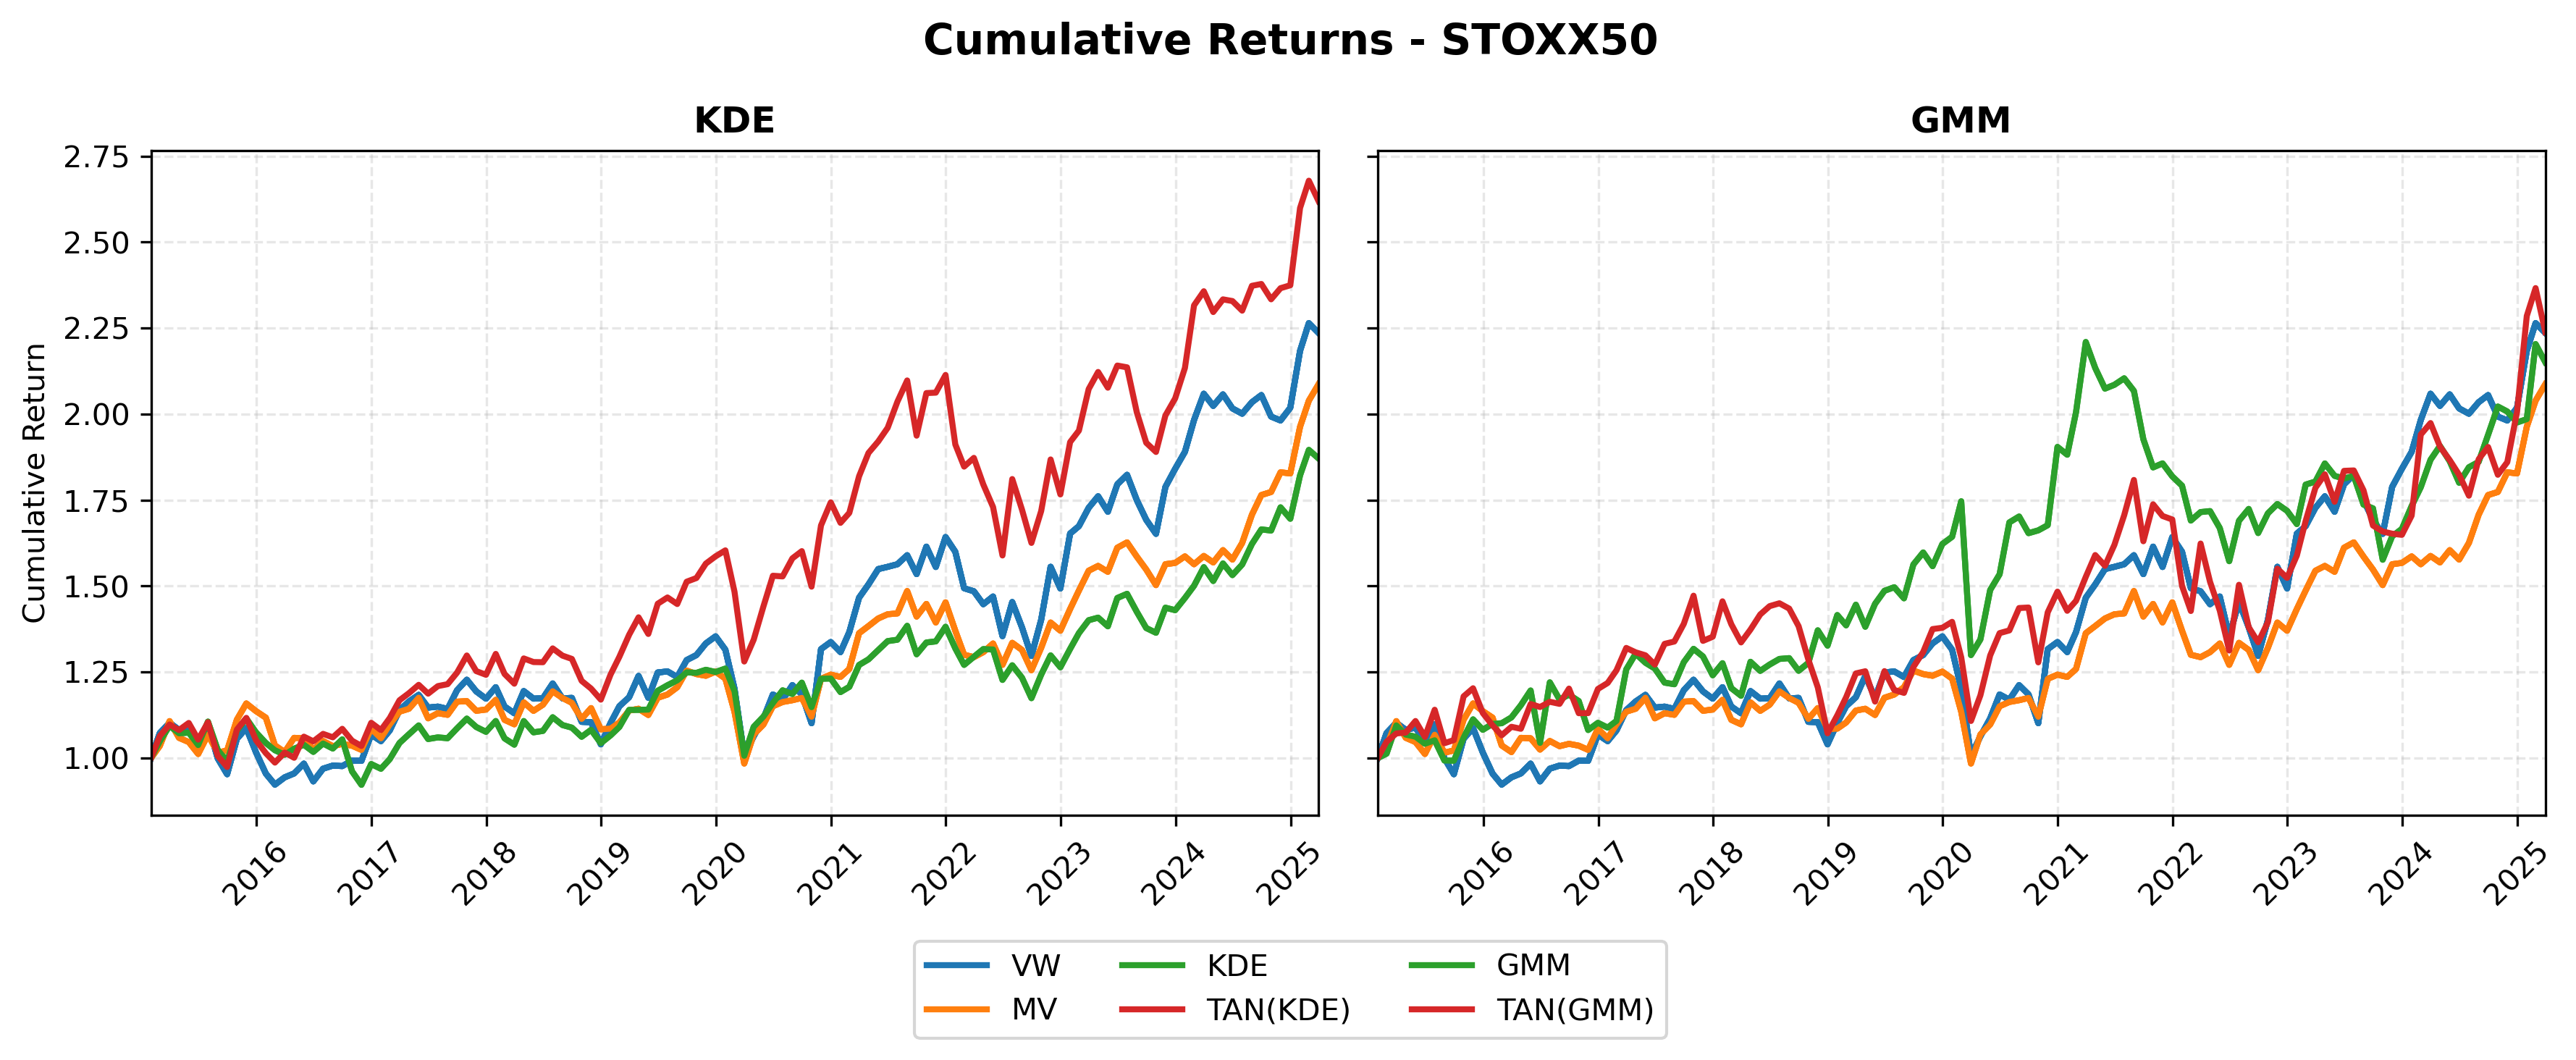
\includegraphics[width=\textwidth]{images/40_9.png}
  \end{minipage}
  \caption[Global best configuration - STOXX50 - Cumulative returns]{Cumulative returns (Jan 2015-Mar 2025) of the best global configuration per strategy on the STOXX50 index. Same layout as Figure \ref{fig:combined6}.}
  \label{fig:combined9}
  \end{center}
  \end{figure}

In the STOXX 50, the VW portfolio delivered middle-of-the-pack results across all metrics. At the same time, MV once again achieved the lowest volatility but also recorded a comparatively high drawdown. 

The KDE portfolio performed similarly to VW, with slightly lower volatility and a deeper and longer drawdown. The TAN(KDE) portfolio was the strongest overall performer, ranking first in cumulative and risk-adjusted returns and drawdown management. It also achieved the second-best $VaR$, second only to MV.

The standard GMM portfolio struggled, achieving one of the lowest Sharpe ratios and elevated volatility, although its maximum drawdown was marginally smaller than MV's. The TAN(GMM) variant proved more successful, essentially a higher volatility variant of VW. However, unlike KDE, its extra volatility did not translate into deeper drawdowns, which were among the shallowest, albeit with longer durations.

\subsection{Overview}
The preceding analysis aimed to compare the consistency and adaptability of various portfolio construction approaches to varying market regimes. The results underscore that while no single strategy dominates universally, certain approaches exhibit more reliable performance characteristics than others.

The VW portfolio demonstrates remarkable robustness, achieving the highest penalized Sharpe Ratio overall. This finding reinforces the challenge of consistently outperforming simple market-cap weighting when accounting for strategy stability across markets. The VW approach benefits from its simplicity and absence of estimation error, delivering competitive performance without the parameter sensitivity that affects more complex methods.

The MV portfolio also performs admirably, particularly in risk management, consistently delivering low volatility across most indices while maintaining competitive Sharpe Ratios. This highlights the enduring value of variance minimization as a portfolio construction technique, especially for risk-averse investors.

Among the density-based approaches, KDE portfolios show greater consistency than their GMM counterparts. The TAN(KDE) portfolio performs particularly well, achieving the second-highest raw Sharpe Ratio overall and demonstrating adaptability across indices. This suggests kernel density estimation provides a more stable foundation for portfolio optimization in diverse market conditions, likely due to its non-parametric nature and reduced sensitivity to outliers.

The GMM-based strategies exhibit the most variable performance across indices. While GMM achieved exceptional results in the S\&P500, its performance was inconsistent in other markets. When applied to sparse data, the anomalously high returns in the S\&P500 raise questions about model stability. This variability suggests that GMM approaches may be more sensitive to market-specific characteristics and data conditions, making them less reliable as globally portable strategies without careful calibration.

The index-specific analysis reveals how market structure influences strategy performance. In the highly concentrated HSI, MV significantly outperformed VW, while in the more diversified S\&P500, VW delivered exceptional results. While data-heavy density-based approaches can outperform traditional methods, they do not consistently dominate across all market environments. The VW and MV portfolios remain compelling due to their simplicity and reliability. For practitioners seeking to implement density-based approaches, KDE offers a more stable foundation than GMM, particularly when constructing tangency portfolios.

This section highlights the importance of rigor in strategy selection, especially for investors operating across multiple markets. The choice of optimal strategy and configuration should focus on specific characteristics of the target market, rather than the global performance metrics. In the following sections, we focus on the optimal configuration selection per index and attempt to provide heuristics for future practitioners.

\section{Local Configuration Optima}
\label{sec:localoptima}

Next, we explore how well the strategies perform when the best index-specific configuration is selected. We will once again employ the penalized Sharpe Ratio as our selection criterion for the optimal parameters. Additionally, in this section, we will display cumulative returns of subsampled configurations, if the optimum does not turn out to be to invest in the entirety of the index.

This analysis focuses on median cumulative returns as a measure of central tendency across multiple iterations. For the cumulative return plots, certain portfolios are displayed with an envelope representing the 5\% and 95\% quantiles of the cumulative return series for that configuration.

It's worth noting that it was this local analysis that lead us to identify a performance stability issue. The dominant configurations for MAR and KDE in the S\&P500 presented extremely high cumulative returns and a wide min-max quantile dispersion. With as few as six observations of monthly returns to determine weights for 450 assets, the ratio of observations-to-assets for these configurations was only 1.3\%. This over-performance, coupled with the data sparsity, led us to question the statistical validity of these results. Therefore, we elected to exclude all configurations with an observation-to-asset ratio below 10\% from all empirical analysis in this thesis. This decision is discussed in more detail in Section \ref{sec:limitations}.

\vspace{10mm}
\begin{table}[H]
  \centering
  \begin{table}[H]
  \centering
  \small
  \renewcommand{\arraystretch}{0.9}
  \setlength{\tabcolsep}{3pt}
  % preamble: \usepackage{tabularx,booktabs}
  %           \newcolumntype{Y}{>{\centering\arraybackslash}X}
  \begin{tabularx}{\textwidth}{llccccYYYYYYY}
  \toprule
    &  & \multicolumn{4}{c}{Configuration} & \multicolumn{7}{c}{Metrics} \\
  \cmidrule(lr){3-6} \cmidrule(lr){7-13}
    Index & Strategy & Reb. & Wnd. & Data & N & CR & SR & SR$_p$ & VaR & DD & \textbar DD\textbar & Disp. \\
  \midrule
    \multirow{8}{*}{\textbf{FTSE100}} & VW & monthly & 36 & monthly & 30 & 2.00 & 0.46 & 0.40 & \textbf{0.18} & 0.27 & 2.14 & \textbf{0.46} \\
     & MV & annual & 36 & monthly & 30 & 2.09 & 0.47 & 0.37 & 0.18 & 0.26 & 1.93 & 0.92 \\
     & MAR & annual & 6 & weekly & 30 & \textbf{2.69} & 0.53 & 0.35 & 0.29 & 0.41 & 3.13 & 2.66 \\
     & TAN & annual & 120 & monthly & 30 & 2.19 & 0.47 & 0.33 & 0.21 & 0.23 & 2.36 & 1.31 \\
     & KDE & annual & 36 & monthly & 30 & 2.38 & \textbf{0.59} & \textbf{0.43} & 0.18 & \textbf{0.20} & \textbf{1.90} & 1.46 \\
     & GMM & annual & 6 & monthly & 30 & 2.24 & 0.50 & 0.30 & 0.22 & 0.31 & 3.65 & 2.45 \\
     & TAN(KDE) & annual & 3 & weekly & 30 & 2.33 & 0.49 & 0.36 & 0.23 & 0.37 & 2.34 & 1.50 \\
     & TAN(GMM) & annual & 3 & weekly & 30 & 2.25 & 0.45 & 0.29 & 0.25 & 0.37 & 3.21 & 1.98 \\
  \midrule
    \multirow{8}{*}{\textbf{HSI}} & VW & annual & 60 & daily & 20 & 1.55 & 0.24 & 0.16 & 0.30 & 0.41 & 5.08 & 0.76 \\
     & MV & monthly & 3 & daily & 30 & 2.43 & \textbf{0.62} & \textbf{0.56} & \textbf{0.20} & \textbf{0.28} & 3.99 & \textbf{0.50} \\
     & MAR & annual & 12 & daily & 30 & 2.17 & 0.40 & 0.31 & 0.31 & 0.42 & 4.94 & 1.11 \\
     & TAN & monthly & 12 & daily & 30 & \textbf{2.87} & 0.54 & 0.42 & 0.32 & 0.39 & 3.23 & 2.16 \\
     & KDE & monthly & 3 & daily & 30 & 2.25 & 0.53 & 0.47 & 0.22 & 0.30 & 4.14 & 0.54 \\
     & GMM & monthly & 6 & daily & 30 & 1.96 & 0.38 & 0.25 & 0.26 & 0.43 & 4.58 & 1.42 \\
     & TAN(KDE) & monthly & 12 & daily & 30 & 2.80 & 0.54 & 0.41 & 0.31 & 0.39 & 3.20 & 2.30 \\
     & TAN(GMM) & monthly & 6 & weekly & 30 & 2.26 & 0.44 & 0.31 & 0.29 & 0.37 & \textbf{3.13} & 1.79 \\
  \midrule
    \multirow{8}{*}{\textbf{S\&P500}} & VW & annual & 120 & monthly & 450 & 3.40 & 0.86 & 0.85 & 0.23 & 0.23 & \textbf{1.50} & \textbf{0.07} \\
     & MV & monthly & 3 & daily & 100 & 2.49 & 0.67 & 0.57 & \textbf{0.18} & 0.26 & 1.89 & 1.08 \\
     & MAR & annual & 120 & monthly & 450 & \textbf{5.55} & 0.95 & 0.88 & 0.26 & 0.33 & 1.95 & 1.95 \\
     & TAN & annual & 120 & monthly & 450 & 4.26 & \textbf{0.99} & \textbf{0.89} & 0.24 & 0.19 & 1.85 & 3.04 \\
     & KDE & monthly & 120 & monthly & 450 & 3.73 & 0.83 & 0.68 & 0.24 & 0.19 & 1.79 & 2.86 \\
     & GMM & monthly & 120 & monthly & 450 & 4.05 & 0.83 & 0.68 & 0.23 & 0.22 & 2.05 & 2.85 \\
     & TAN(KDE) & annual & 120 & monthly & 450 & 3.56 & 0.90 & 0.85 & 0.23 & 0.20 & 1.76 & 0.60 \\
     & TAN(GMM) & monthly & 120 & monthly & 450 & 4.84 & 0.95 & 0.82 & 0.25 & \textbf{0.19} & 1.75 & 3.23 \\
  \midrule
    \multirow{8}{*}{\textbf{STOXX50}} & VW & annual & 3 & monthly & 30 & 2.43 & 0.49 & 0.45 & \textbf{0.23} & \textbf{0.25} & 1.71 & \textbf{0.45} \\
     & MV & annual & 60 & daily & 30 & 3.02 & \textbf{0.67} & \textbf{0.58} & 0.24 & 0.33 & 1.70 & 1.19 \\
     & MAR & annual & 12 & daily & 30 & \textbf{3.23} & 0.63 & 0.51 & 0.31 & 0.40 & 2.06 & 2.53 \\
     & TAN & annual & 12 & daily & 30 & 2.94 & 0.57 & 0.45 & 0.30 & 0.39 & 2.39 & 2.02 \\
     & KDE & annual & 6 & daily & 30 & 2.51 & 0.55 & 0.50 & 0.23 & 0.34 & \textbf{1.63} & 0.60 \\
     & GMM & annual & 36 & monthly & 30 & 2.96 & 0.57 & 0.41 & 0.25 & 0.26 & 2.35 & 2.41 \\
     & TAN(KDE) & annual & 36 & monthly & 30 & 3.00 & 0.57 & 0.48 & 0.25 & 0.26 & 1.92 & 1.29 \\
     & TAN(GMM) & annual & 6 & weekly & 20 & 2.85 & 0.52 & 0.38 & 0.33 & 0.37 & 2.61 & 2.49 \\
  \bottomrule
  \end{tabularx}
\end{table}

  \caption[All optimal configurations]{Optimal configuration and end-of-period performance for each strategy by index. For each index and strategy, we report rebalancing frequency (Reb.), lookback window in months (Wnd.), data frequency (Data), and the number of assets in the portfolio (N). Performance metrics: cumulative return (CR), Sharpe ratio (SR), penalized Sharpe ratio (SR$_p$), terminal cumulative return dispersion (Disp.), maximum drawdown (DD), drawdown duration (|DD|), and 95\% Value-at-Risk (VaR); metrics are computed over the 2015-2025 sample. Within each index block, boldface highlights the best value in that column across strategies.}

  \label{tab:single9}
\end{table}

\newpage
We observe that the optimal configurations for MAR consistently generate the highest median cumulative returns (above 5.5 in the S\&P500). This outperformance, however, comes with substantially higher dispersion, often at or above 2.5. For context, the dispersion values for VW typically remain below 0.5, while MV portfolios range between 0.5 and 1.2. Values above 2.0 suggest a comparatively low strategy stability.

KDE portfolios consistently present a trade-off across markets. They achieve lower dispersion than their MAR counterparts (45-75\% improvement) in all markets but the S\&P500 (45\% increase). However, this stability frequently comes at the cost of lower absolute returns. While KDE sometimes achieves higher Sharpe ratios than MAR, particularly in smaller or less efficient markets, it consistently trails in cumulative returns.

\vspace{5mm}
\begin{figure}[H]
  \begin{center}
  \begin{minipage}{1\textwidth}
    \centering
    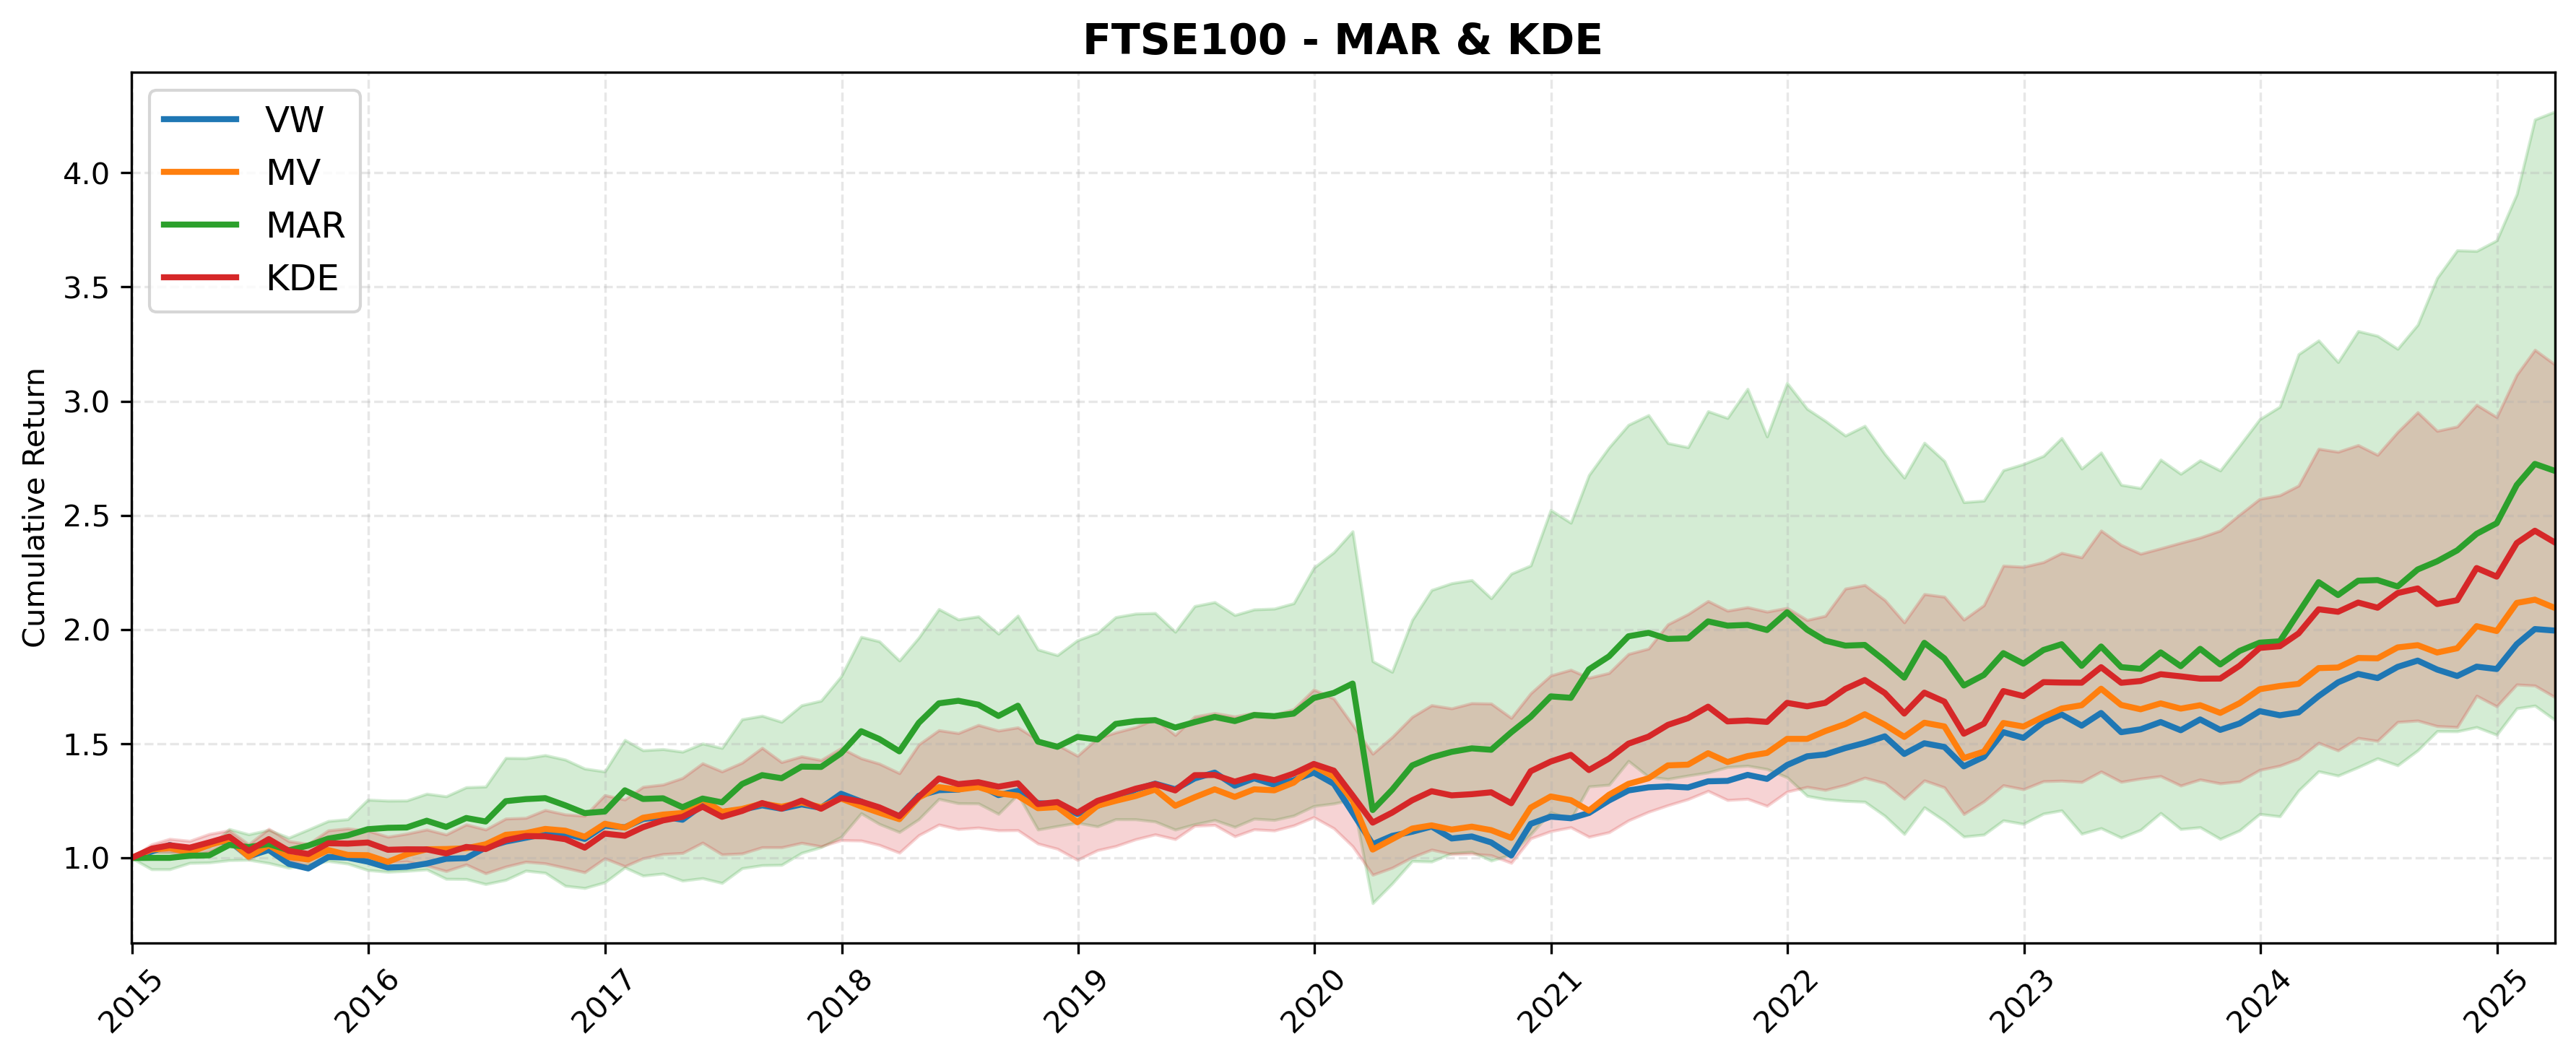
\includegraphics[width=\textwidth]{images/40_10.png}
  \end{minipage}
  \caption[Local best configuration - FTSE100 - Cumulative returns]{Cumulative returns (Jan 2015-Mar 2025) on the FTSE100 index of the locally optimal configuration for each strategy, selected by the highest penalized Sharpe ratio. VW (blue) and MV (orange) show the pointwise median of all cumulative-return paths; MAR (green) and KDE (red) additionally display shaded envelopes spanning the 5th-95th percentiles at each date. All series are normalized to 1.0 at the start date.}
  \label{fig:combined10}
  \end{center}
  \end{figure}

The performance of GMM portfolios also lacks consistency. While occasionally delivering strong performance, GMM typically exhibits high dispersion relative to returns, often matching or exceeding MAR's already elevated dispersion levels. More concerning is GMM's performance variability across different market environments, delivering competitive returns in some markets while significantly underperforming in others.

\begin{figure}[H]
  \begin{center}
  \begin{minipage}{1\textwidth}
    \centering
    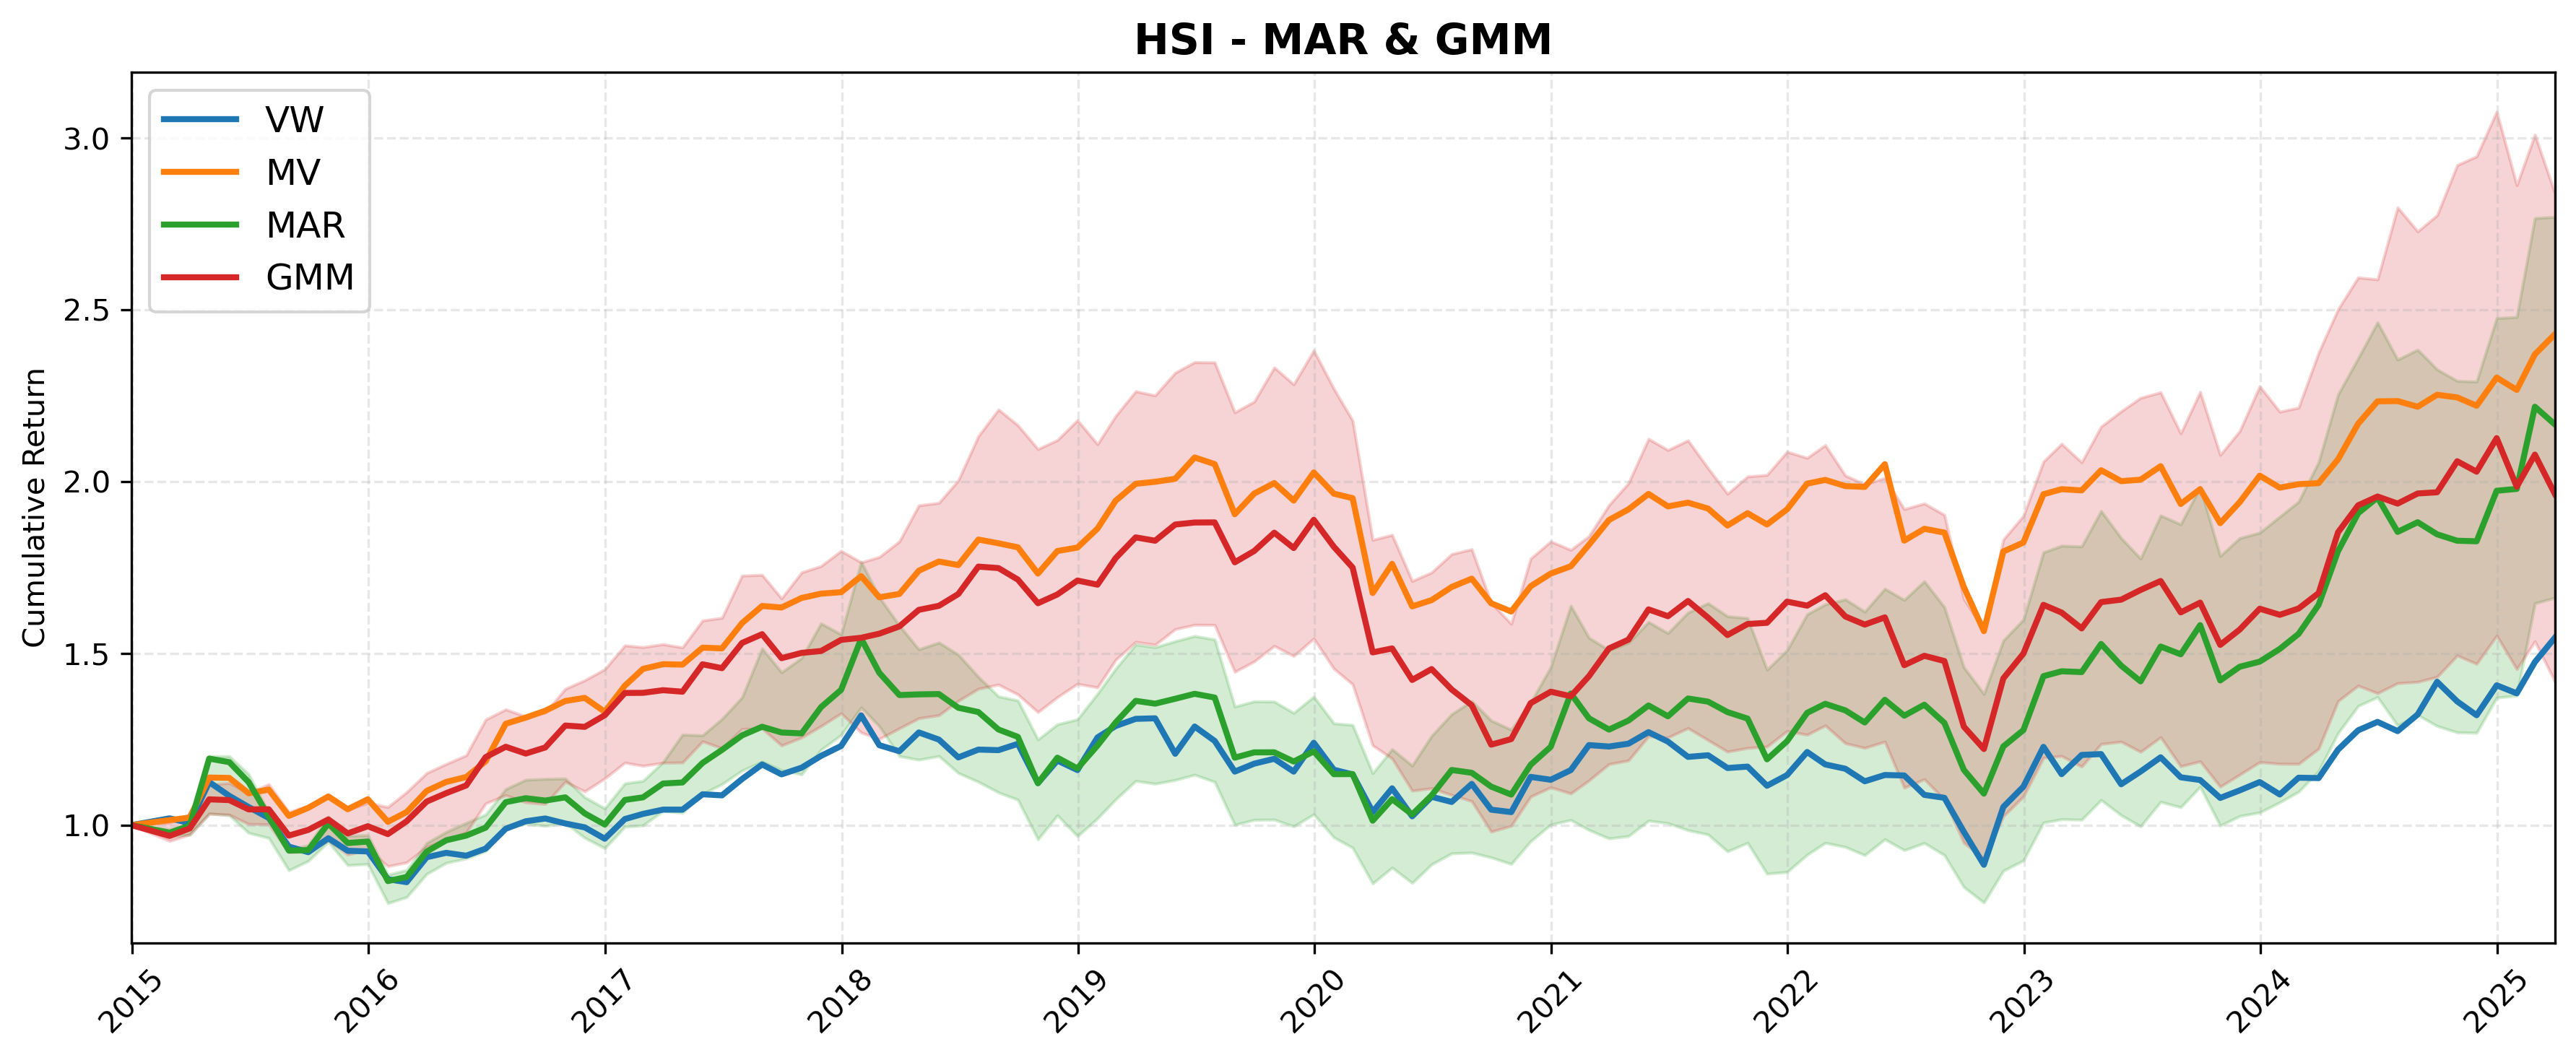
\includegraphics[width=\textwidth]{images/40_11.png}
  \end{minipage}
  \caption[Local best configuration - HSI - Cumulative returns]{Cumulative returns (Jan 2015-Mar 2025) on the HSI index of the locally optimal configuration for each strategy, selected by the highest penalized Sharpe ratio. Identical layout to Figure \ref{fig:combined10}, with the exception that the GMM portfolio (red) is shown instead of KDE.}
  \label{fig:combined11}
  \end{center}
  \end{figure}

KDE shows promise in tangency portfolio construction. TAN(KDE) demonstrates competitive performance with traditional TAN portfolios in terms of the Sharpe ratio, while typically offering lower dispersion. Notably, TAN(KDE) achieves an extremely low comparative dispersion in the S\&P500 of 0.602, lower than that of the MV portfolio. TAN(GMM) shows high return potential but continues to exhibit the highest dispersion values among all strategies, undermining its practical implementation value.

\vspace{5mm}
\begin{figure}[H]
  \begin{center}
  \begin{minipage}{1\textwidth}
    \centering
    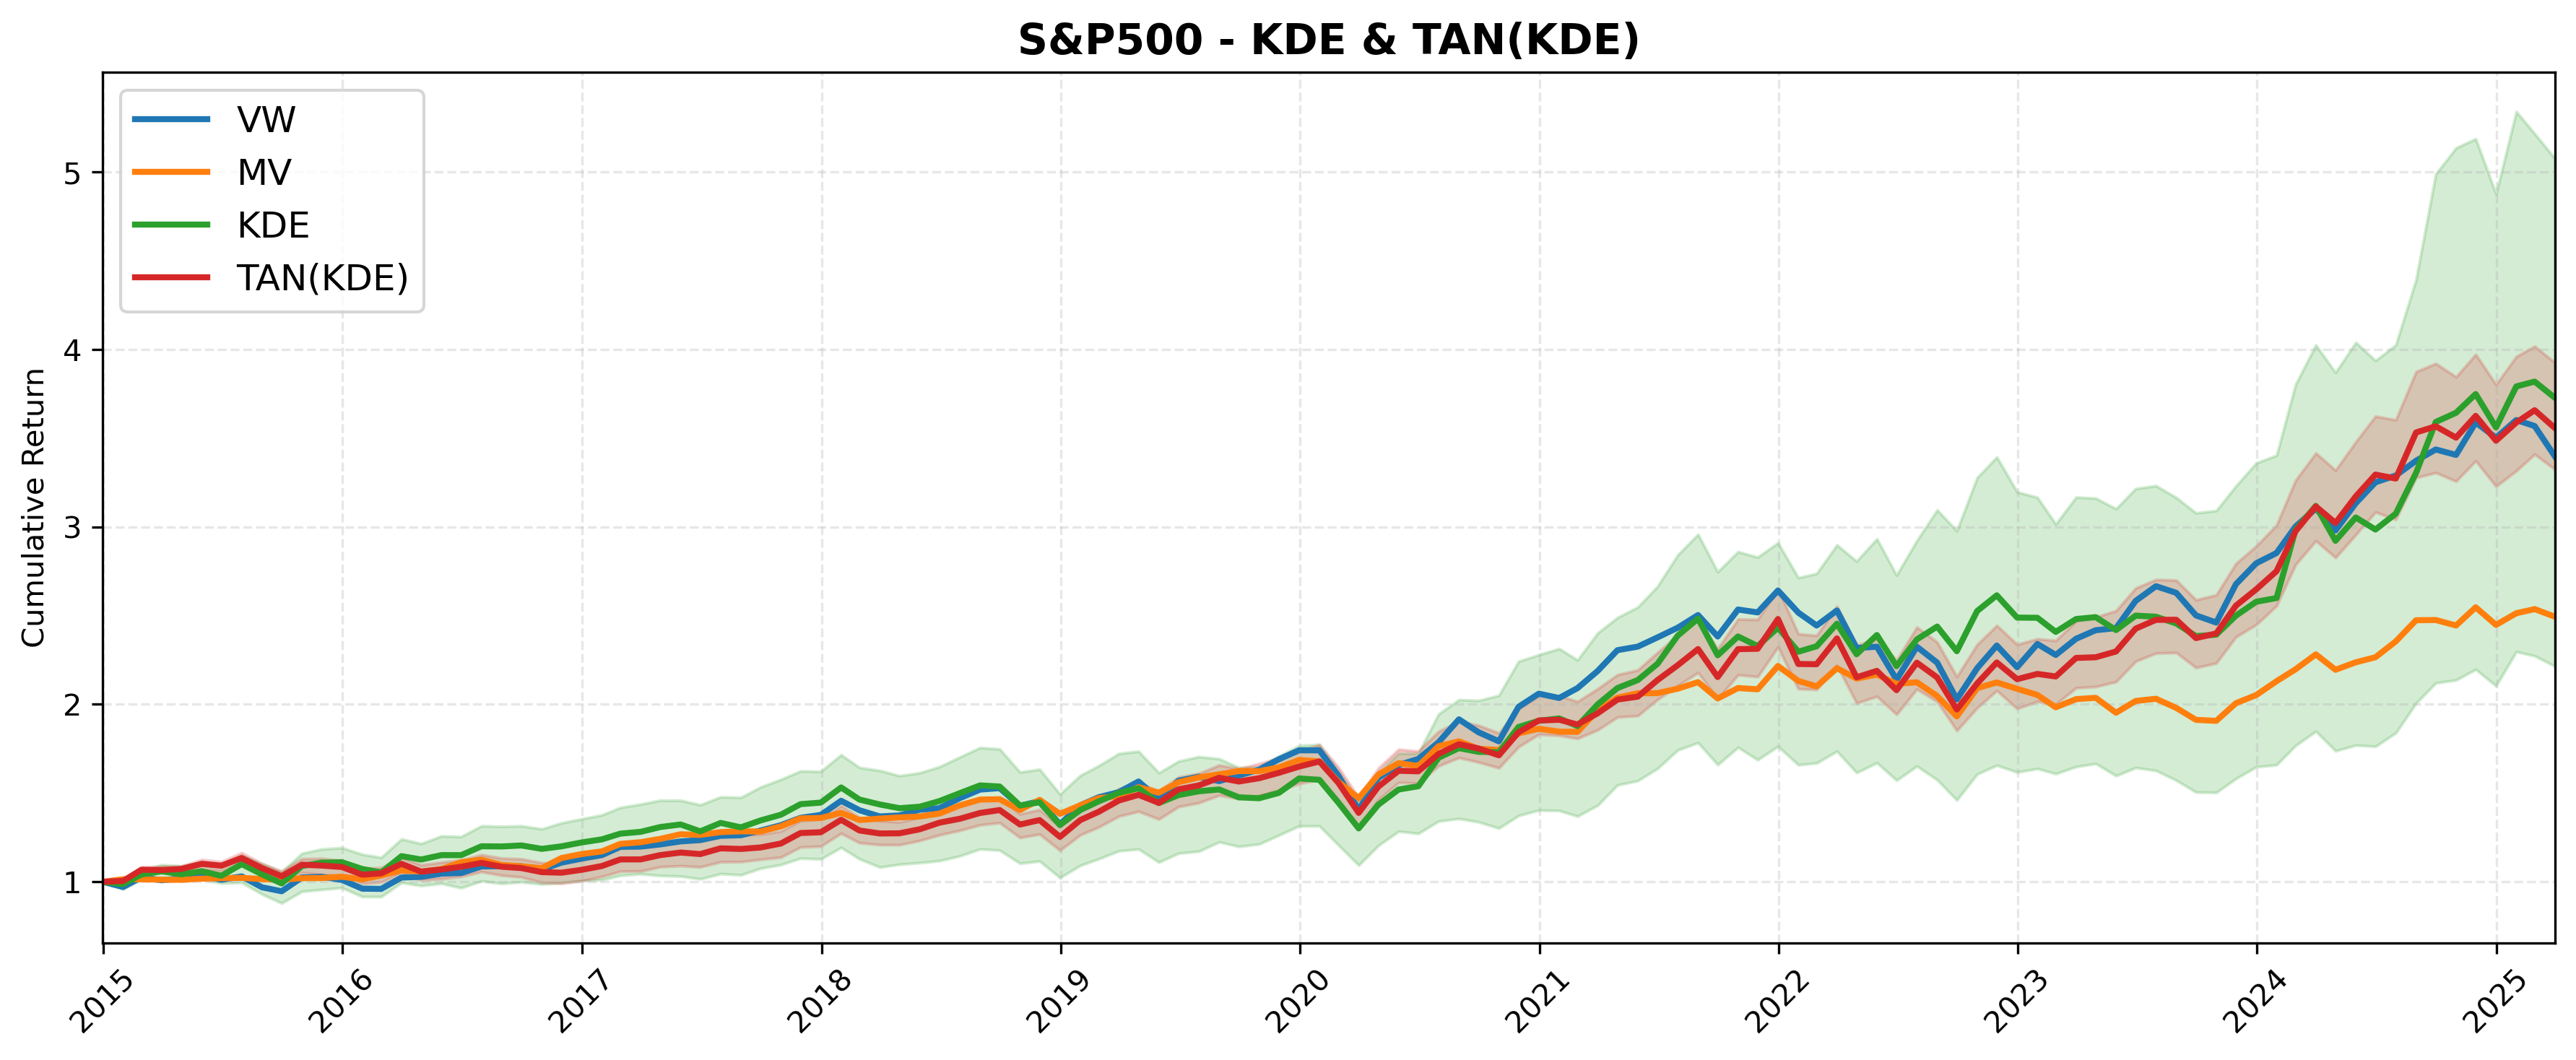
\includegraphics[width=\textwidth]{images/40_12.png}
  \end{minipage}
  \caption[Local best configuration - S\&P500 - Cumulative returns]{Cumulative returns (Jan 2015-Mar 2025) on the S\&P500 index of the locally optimal configuration for each strategy, selected by the highest penalized Sharpe ratio. Identical layout to Figure \ref{fig:combined10}, with the exception that the KDE portfolio (green) is shown instead of MAR, TAN(KDE) (red) instead of KDE.}
  \label{fig:combined12}
  \end{center}
  \end{figure}

The variations in configuration are partly responsible for the performance differences. KDE portfolios favor shorter lookback windows in smaller markets but require longer ones in the S\&P500, likely due to data demands in larger universes. GMM portfolios prefer intermediate windows in some markets and longer ones in others. The relationships between configurations and performance will be further examined in subsequent sections.

Maximum drawdown metrics reveal a more nuanced picture than initially apparent. In several instances, density-based approaches demonstrate superior drawdown protection compared to traditional portfolios. In the S\&P500, TAN(KDE) achieves a maximum drawdown of 20\%, lower than the MV portfolio's 26\%. Similarly, in the FTSE100, KDE records the lowest and shortest maximum drawdown among all strategies at 20\%, significantly outperforming both MAR (41\%) and MV (26\%). This pattern extends to Value-at-Risk measures, where KDE frequently records the lowest or second-lowest VaR figures across indices. The above demonstrates that KDE-based approaches offer enticing downside risk management while maintaining competitive returns.

KDE also demonstrates enhanced estimation stability compared to MAR and more consistent performance across markets than GMM. The advantage is most visible in tangency portfolios: TAN(KDE) matches or exceeds the returns of the traditional TAN while achieving significantly lower dispersion. This stability advantage persists across different market environments, suggesting that non-parametric density estimation adapts to heterogeneous return distributions well.

The rankings in Table \ref{tab:married1} crystallize this result. KDE now tops the overall table, finishing first in four of seven metrics and never worse than third; MV and TAN(KDE) share second place, while both GMM variants are relegated to the bottom of the rankings. In summary, once we equalise scale across markets, KDE emerges as the most consistently attractive strategy, with MV and TAN(KDE) close behind.

\vspace{10mm}
\begin{table}[H]
  \centering
  \begin{tabular}{l|c|*{7}{S[table-format=1.4]}}
  \toprule
  & {Avg. Rank} & {CR} & {SR} & {SR$_p$} & {VaR} & {DD} & {\textbar DD\textbar} & {Disp.} \\
  \midrule
  VW & {4th} & {8th} & {8th} & {6th} & {3rd} & {3rd} & {3rd} & {{\bfseries 1st}} \\
  MV & {{\textit{2nd}}} & {7th} & {5th} & {3rd} & {{\bfseries 1st}} & {2nd} & {4th} & {2nd} \\
  MAR & {6th} & {{\bfseries 1st}} & {{\bfseries 1st}} & {4th} & {8th} & {8th} & {7th} & {5th} \\
  TAN & {5th} & {2nd} & {3rd} & {5th} & {6th} & {6th} & {5th} & {6th} \\
  KDE & {{\bfseries 1st}} & {6th} & {2nd} & {{\bfseries 1st}} & {2nd} & {{\bfseries 1st}} & {{\bfseries 1st}} & {3rd} \\
  GMM & {7th} & {5th} & {6th} & {8th} & {4th} & {5th} & {8th} & {7th} \\
  TAN(KDE) & {{\textit{2nd}}} & {3rd} & {4th} & {2nd} & {5th} & {4th} & {2nd} & {4th} \\
  TAN(GMM) & {8th} & {4th} & {7th} & {7th} & {7th} & {7th} & {6th} & {8th} \\
  \bottomrule
\end{tabular}

  \caption[Optimal strategy ranking]{Relative performance of each strategy after normalising metrics within every index, averaging the normalised scores across the indices, and converting these averages to ordinal ranks (1=best). "Avg.Rank" is the arithmetic mean of the seven column ranks; the overall winner in each column is bold; contested rankings are italicised. Metric definitions are identical to Table \ref{tab:single9}.}
  \label{tab:married1}
\end{table}

\newpage
\section{Where \& Why Do Density-Based Strategies Win?}
% \clearpage
After filtering for stability (observation-to-asset ratio $\geq 10$\%), we assess the 828 remaining portfolio configurations per index. The heat maps in this section compare the differences in $SR_{p}$ or $DD$ between a selected portfolio type and a benchmark, for a given set of configurations. Blue always represents a positive difference (higher $SR_{p}$, lower $DD$), and red - a negative one. 
\vspace{10mm}
\begin{table}[H]
  \centering
  \begin{table}[H]
  \centering
  \setlength{\tabcolsep}{4pt}
  \renewcommand{\arraystretch}{1.0}
  \begin{tabular}{c|l|*{7}{S[table-format=3.2]}}
    Metric & Comparison & \multicolumn{1}{c}{$P(\delta^+)$} & \multicolumn{1}{c}{$E[\delta]$} & \multicolumn{1}{c}{$E[\delta^+]$} & \multicolumn{1}{c}{$E[\delta^-]$} & \multicolumn{1}{c}{$\max(\delta^+)$} & \multicolumn{1}{c}{$\min(\delta^-)$} \\
    \midrule
    \multirow{8}{*}{\textbf{SR$_p$}} & KDE - VW & 0.18 & -0.09 & 0.09 & -0.13 & 0.42 & -0.54 \\
    & KDE - MAR & 0.59 & 0.03 & 0.13 & -0.10 & 0.53 & -0.50 \\
    & TAN(KDE) - VW & 0.20 & -0.08 & 0.08 & -0.12 & 0.40 & -0.49 \\
    & TAN(KDE) - TAN & 0.83 & 0.02 & 0.03 & -0.02 & 0.20 & -0.16 \\
    \cmidrule[0.4pt]{2-2}
    & GMM - VW & 0.07 & -0.21 & 0.08 & -0.23 & 0.34 & -0.94 \\
    & GMM - MAR & 0.33 & -0.08 & 0.09 & -0.16 & 0.43 & -0.75 \\
    & TAN(GMM) - VW & 0.09 & -0.19 & 0.11 & -0.22 & 0.52 & -0.85 \\
    & TAN(GMM) - TAN & 0.15 & -0.09 & 0.03 & -0.11 & 0.26 & -0.68 \\
    \midrule
    \multirow{4}{*}{\textbf{DD}} & KDE - MV & 0.46 & -0.00 & 0.03 & -0.03 & 0.17 & -0.20 \\
    & TAN(KDE) - MV & 0.25 & -0.03 & 0.05 & -0.06 & 0.22 & -0.26 \\
    \cmidrule[0.4pt]{2-2}
    & GMM - MV & 0.07 & -0.07 & 0.03 & -0.07 & 0.17 & -0.34 \\
    & TAN(GMM) - MV & 0.09 & -0.09 & 0.04 & -0.10 & 0.18 & -0.34 \\
  \end{tabular}
\end{table}

  \caption[Metric comparison across all configurations]{Summary statistics for the performance difference $\delta$ between each strategy and its benchmark, across all stable window-rebalancing configurations. Two metrics are shown: inverted maximum drawdown (DD) and penalized Sharpe ratio (SR$_p$). For each Metric-Comparison pair, $P(\delta^+)$ is the proportion with positive $\delta$ (i.e.\ strategy improves over the benchmark), $E[\delta]$ is the mean increase, $E[\delta^+]$ and $E[\delta^-]$ are the mean positive and negative deviations, and $\max(\delta^+)$, $\min(\delta^-)$ give the largest increase and largest shortfall, respectively. 828 configurations per portfolio pair are compared.}
  \label{tab:single10}
\end{table}

Table \ref{tab:single10} is an aggregate of all stable configuration comparisons. The heatmap grids that follow, however, present this information per index, hence the slightly different ranges of values in Figures \ref{fig:combined13} to \ref{fig:combined17}.

\begin{figure}[H]
  \begin{center}
  \begin{minipage}{1\textwidth}
    \centering
    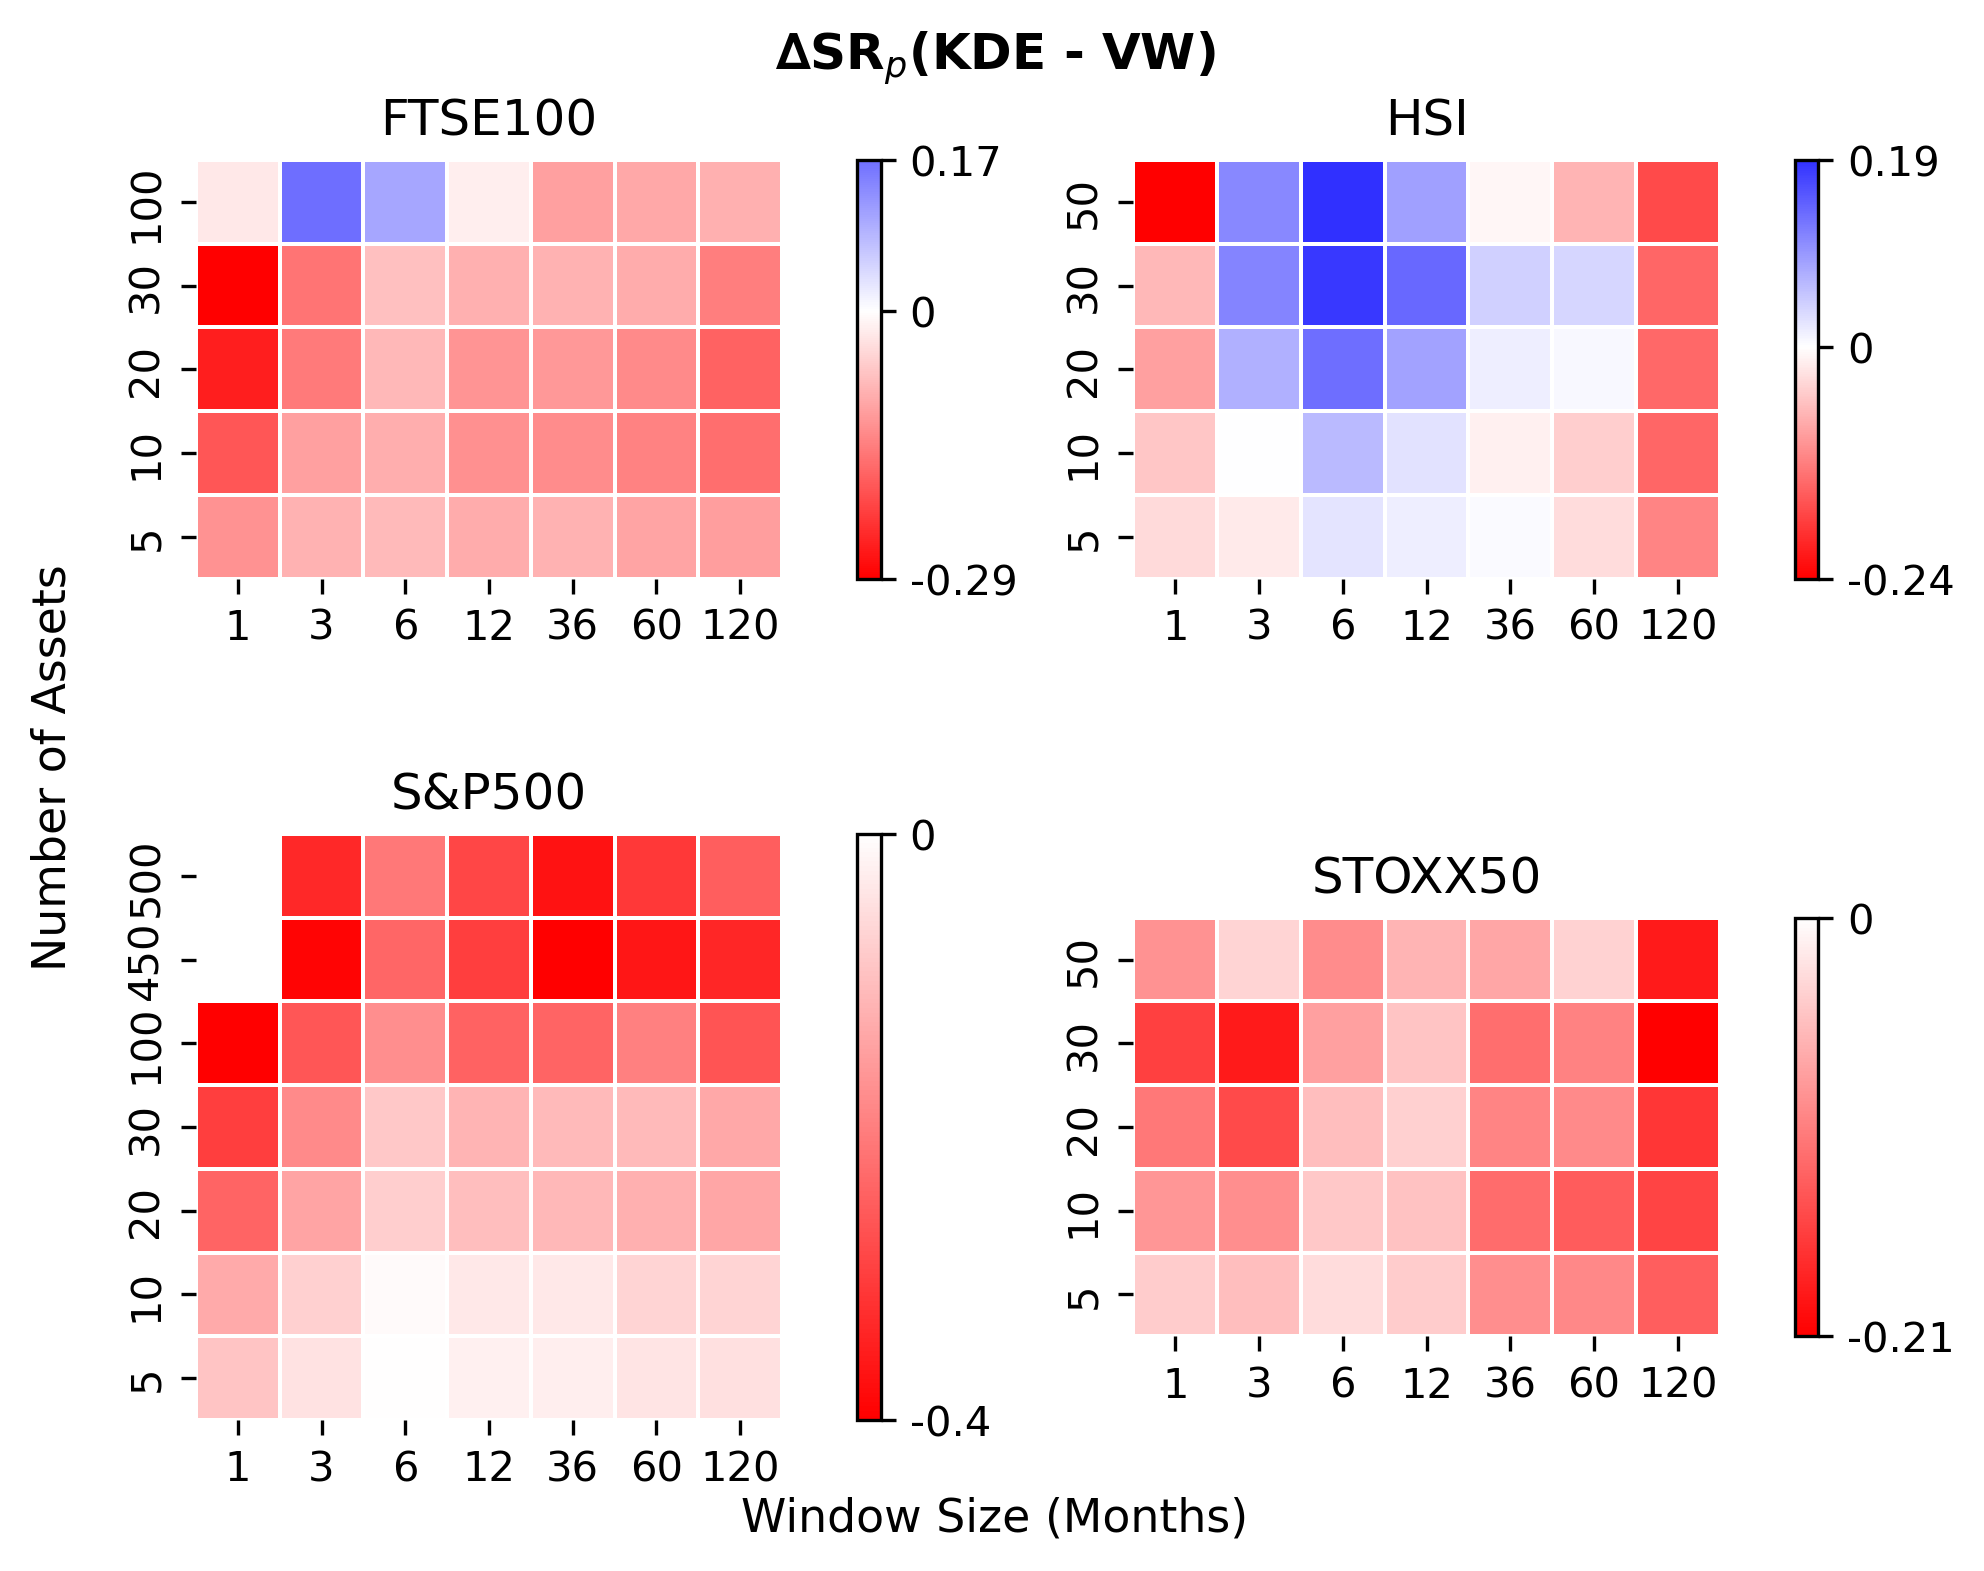
\includegraphics[width=\textwidth]{images/40_14.png}
  \end{minipage}
  \caption[Heatmap 1]{Diverging-color heatmaps of the penalized Sharpe-ratio difference $\Delta SR_p = SR_p(\mathrm{KDE}) - SR_p(\mathrm{VW})$ across model configurations. Each panel shows one index (FTSE100, HSI, S\&P500, STOXX50), with a lookback window (months) on the x-axis and number of assets in the portfolio on the y-axis. Cell color follows a two-slope norm centered at zero. Blue always represents an improvement; red always represents a shortfall. The side color bars indicate the mapping of $\Delta SR_p$ values.}
  \label{fig:combined13}
  \end{center}
  \end{figure}

Compared to the VW portfolio, vanilla KDE outperforms in only 18\% of the grid, with a mean uplift of +9\% in penalized Sharpe Ratio and a mean shortfall of -13\% when it underperforms. Notably, this overperformance comes mainly from the HSI index, clustered around a 6-month data window with approximately 50 assets. A similar comparison performed below with GMM leads us to believe that this is not necessarily a sign of the aptitude of parametric models in that market, but rather a sign of the inaptitude of the VW portfolio.

Comparing against the MAR portfolio raises KDE's win-rate to 59\%, which is especially pronounced for lookback windows of 12 months or less, with an average $SR_{p}$ gain of +13\%. This advantage gradually wanes as the number of assets expands toward full-index universes.

\begin{figure}[H]
  \begin{center}
  \begin{minipage}{1\textwidth}
    \centering
    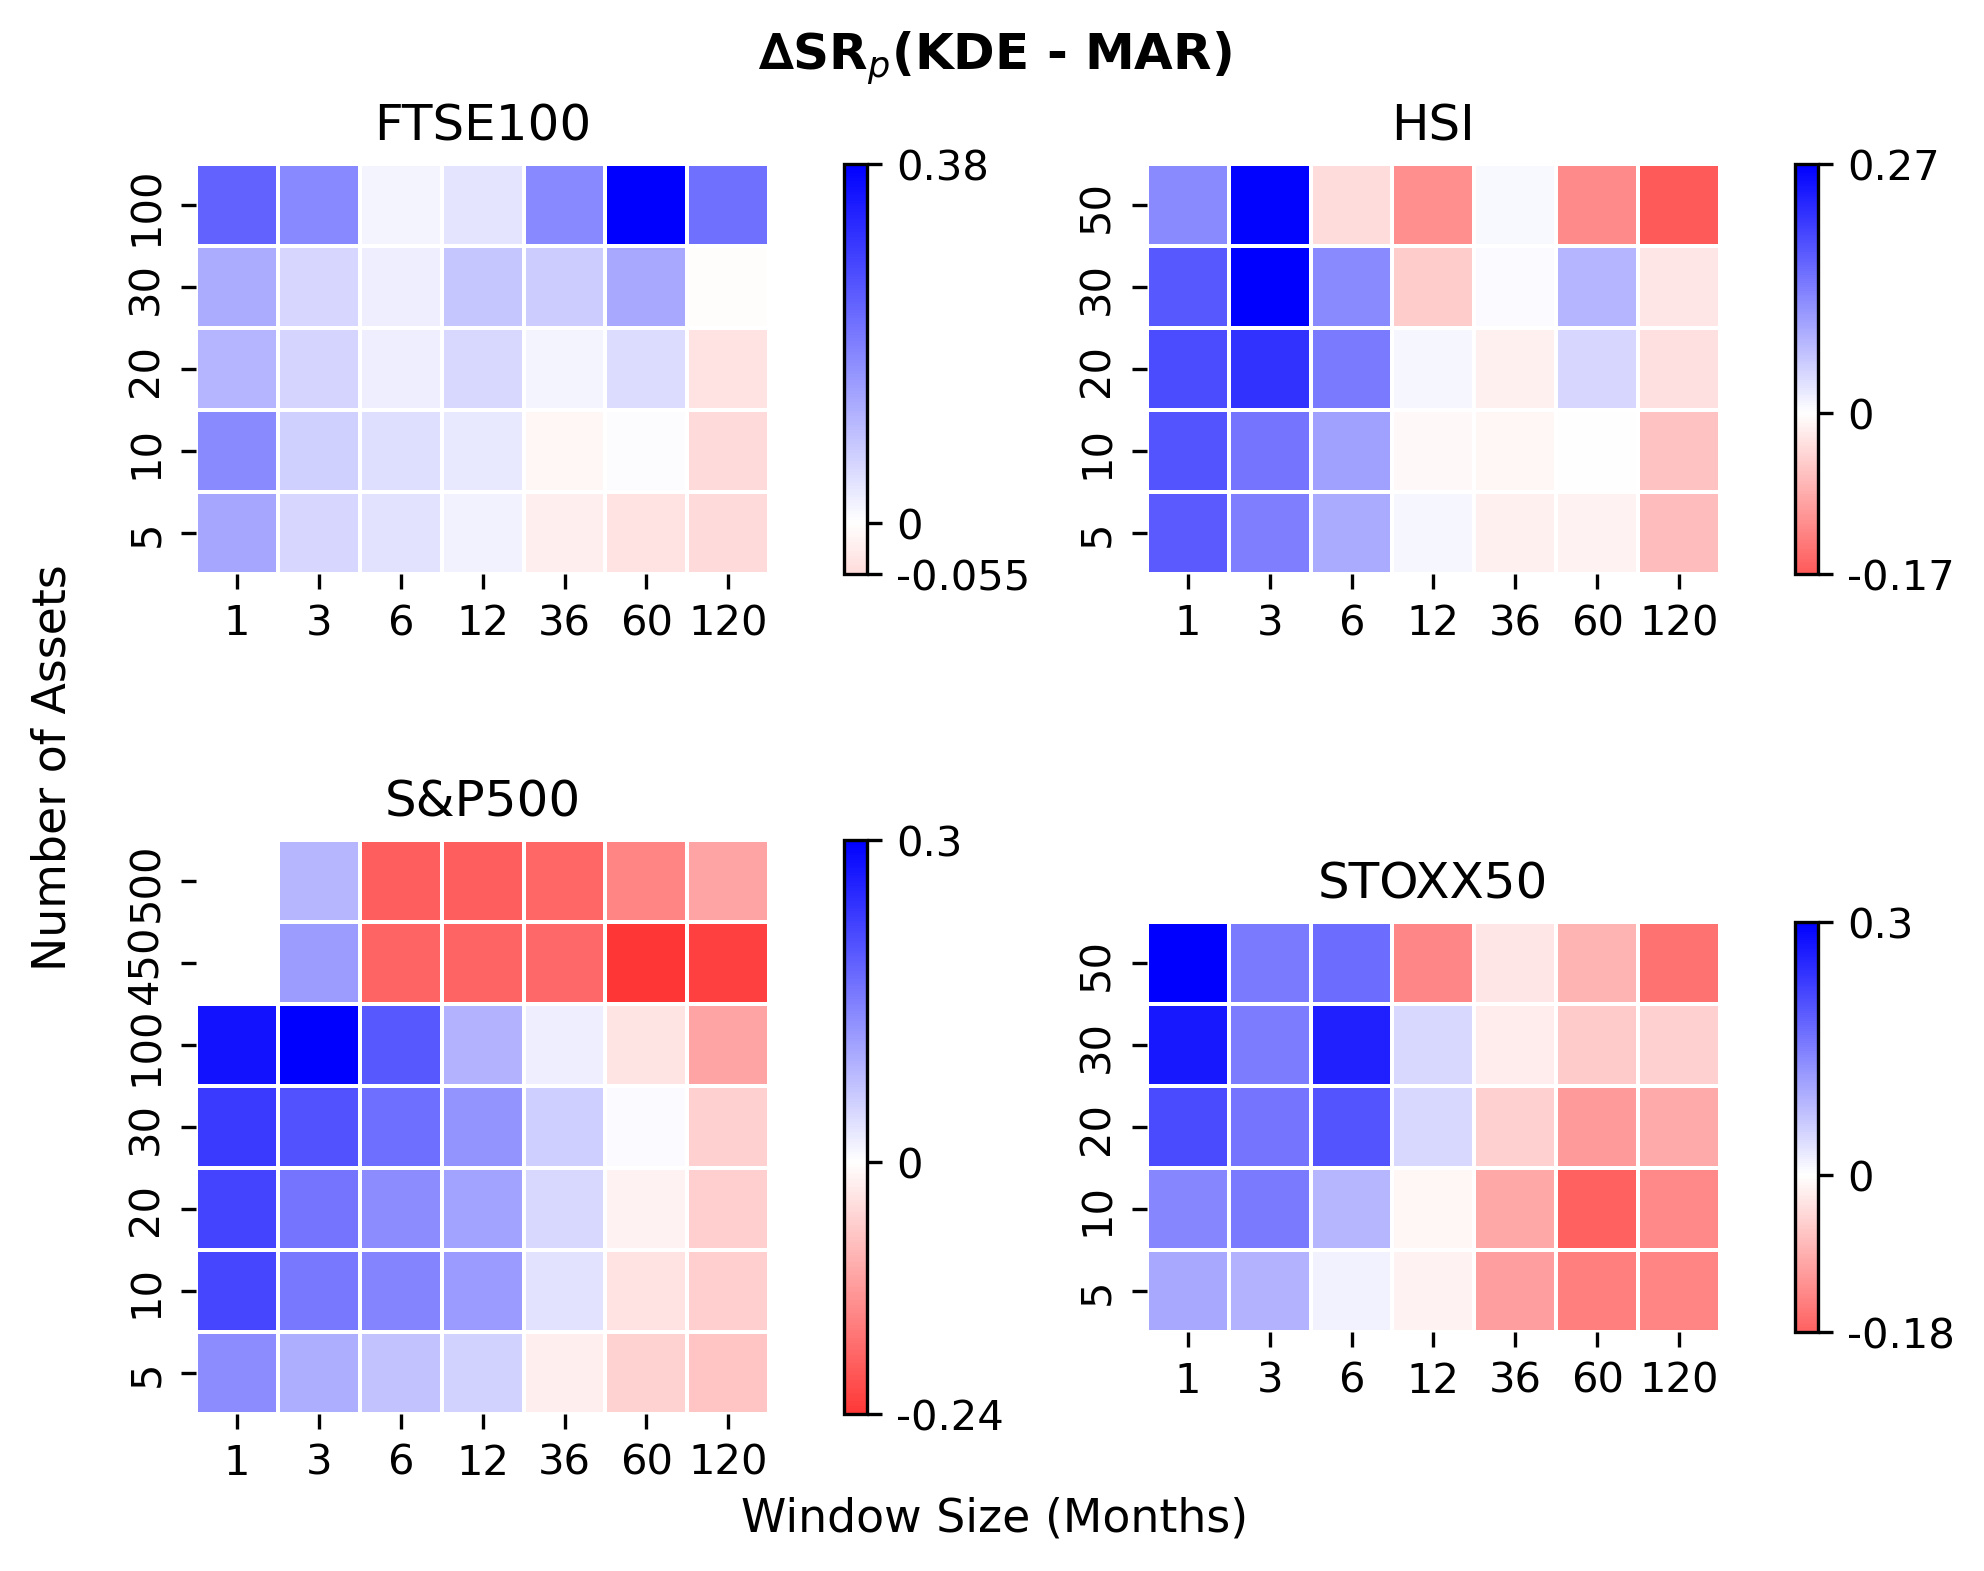
\includegraphics[width=\textwidth]{images/40_15.png}
  \end{minipage}
  \caption[Heatmap 2]{Diverging-color heatmaps of the penalized Sharpe-ratio difference $\Delta SR_p = SR_p(\mathrm{KDE}) - SR_p(\mathrm{MAR})$ across model configurations. Otherwise identical to Figure \ref{fig:combined13}.}
  \label{fig:combined14}
  \end{center}
  \end{figure}

The tangency variant of KDE yields the highest improvements in terms of $SR_{p}$. TAN(KDE) exceeds the classic tangency portfolio in 83\% of configurations, delivering an improvement of +3\%, and a decrease of -2\% on average. This consistency holds across both monthly and annual rebalancing frequencies, window sizes, and numbers of investable assets.

\begin{figure}[H]
  \begin{center}
  \begin{minipage}{1\textwidth}
    \centering
    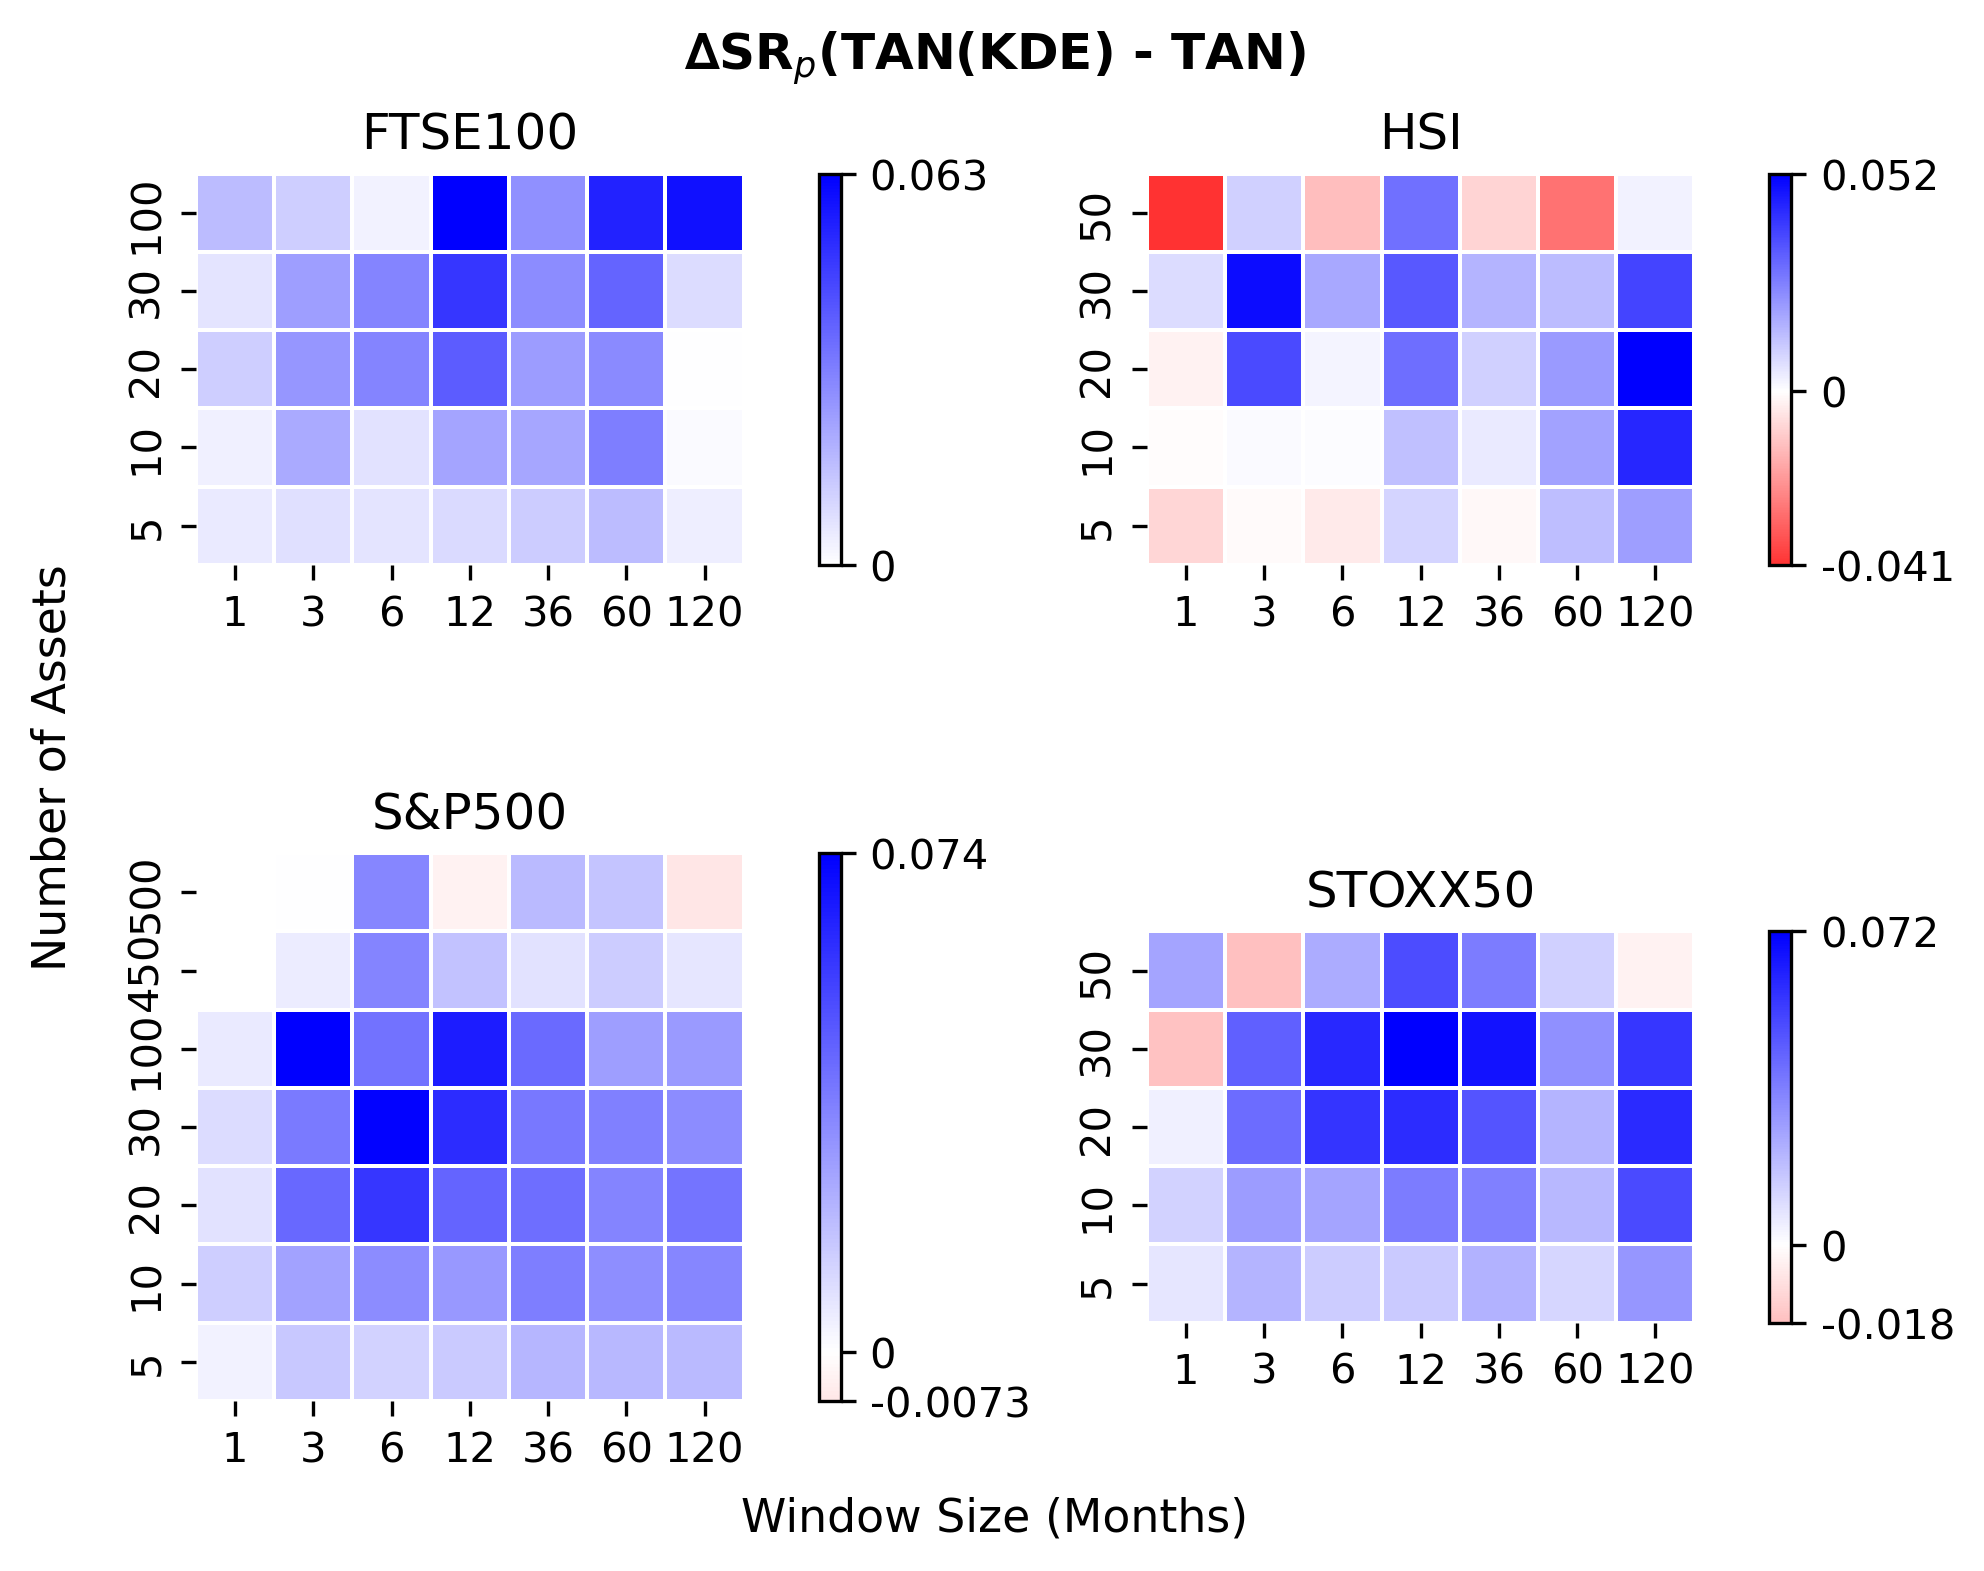
\includegraphics[width=\textwidth]{images/40_16.png}
  \end{minipage}
  \caption[Heatmap 3]{Diverging-color heatmaps of the maximum drawdown difference $\Delta \text{DD} = \text{DD}(\mathrm{KDE}) - \text{DD}(\mathrm{MV})$ across model configurations. A blue cell indicates a decrease in drawdown. Otherwise identical to Figure \ref{fig:combined13}.}
  \label{fig:combined15}
  \end{center}
  \end{figure}

KDE mildly underperforms the MV on maximum drawdown. It reduces $DD$ in 46\% of cases by 3\% points on average, with modest peak improvements at 17\%. TAN(KDE) wins only 25\% of the time but, when successful, can improve drawdown mitigation by 22\% points. Over- and underperformance clusters in certain configuration regions, but this varies by index. Therefore, the choice between KDE-type or MV strategies should be tuned to the market if downside protection is the objective.

\begin{figure}[H]
  \begin{center}
  \begin{minipage}{1\textwidth}
    \centering
    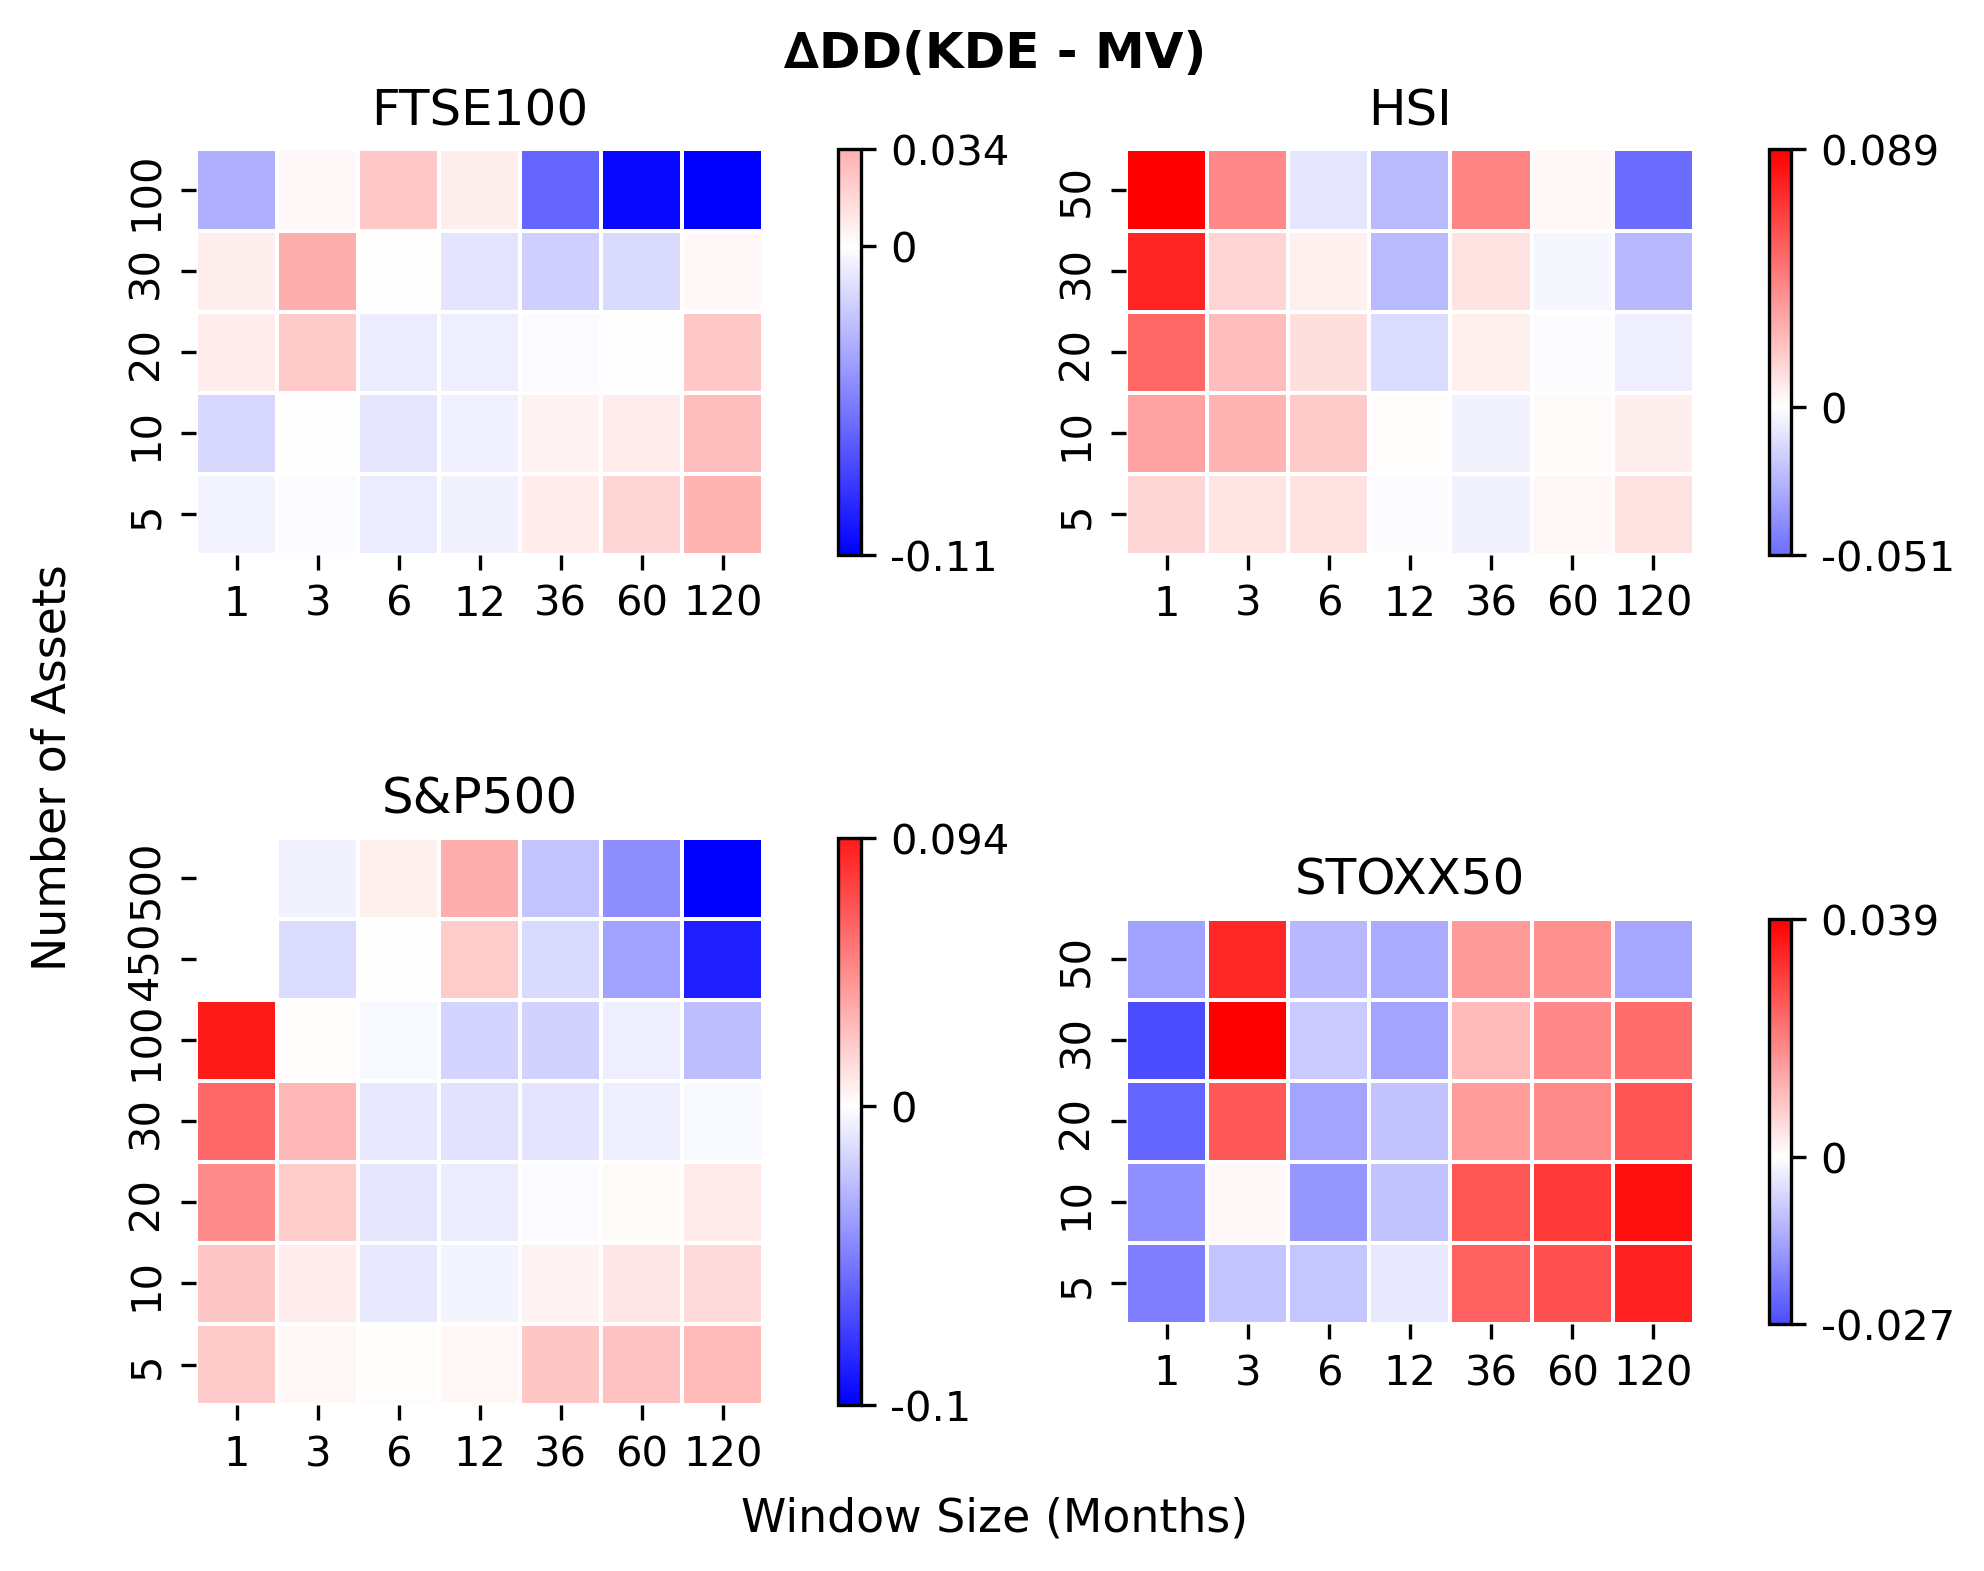
\includegraphics[width=\textwidth]{images/40_17.png}
  \end{minipage}
  \caption[Heatmap 4]{Diverging-color heatmaps of the penalized Sharpe-ratio difference $\Delta SR_p = SR_p(\mathrm{TAN(KDE)}) - SR_p(\mathrm{TAN})$ across model configurations. Otherwise identical to Figure \ref{fig:combined13}.}
  \label{fig:combined16}
  \end{center}
  \end{figure}

Both GMM flavors underperform nearly universally. GMM beats VW by $SR_{p}$ in only 7\% of configurations, and TAN(GMM) in 15\%. Both worsen drawdowns versus MV in over 90\% of configurations. On average, the $DD$ is inflated by 7\% points, while the mean reduction is only 3\% points. The lone "blue" patch appears for TAN(GMM) in the HSI, where, as we noted previously, it is likely that VW itself struggles. We believe that VW's underperformance is the most probable explanation, since the clusters of overperformance for both KDE and GMM are almost exactly in the same configuration region.

\begin{figure}[H]
  \begin{center}
  \begin{minipage}{1\textwidth}
    \centering
    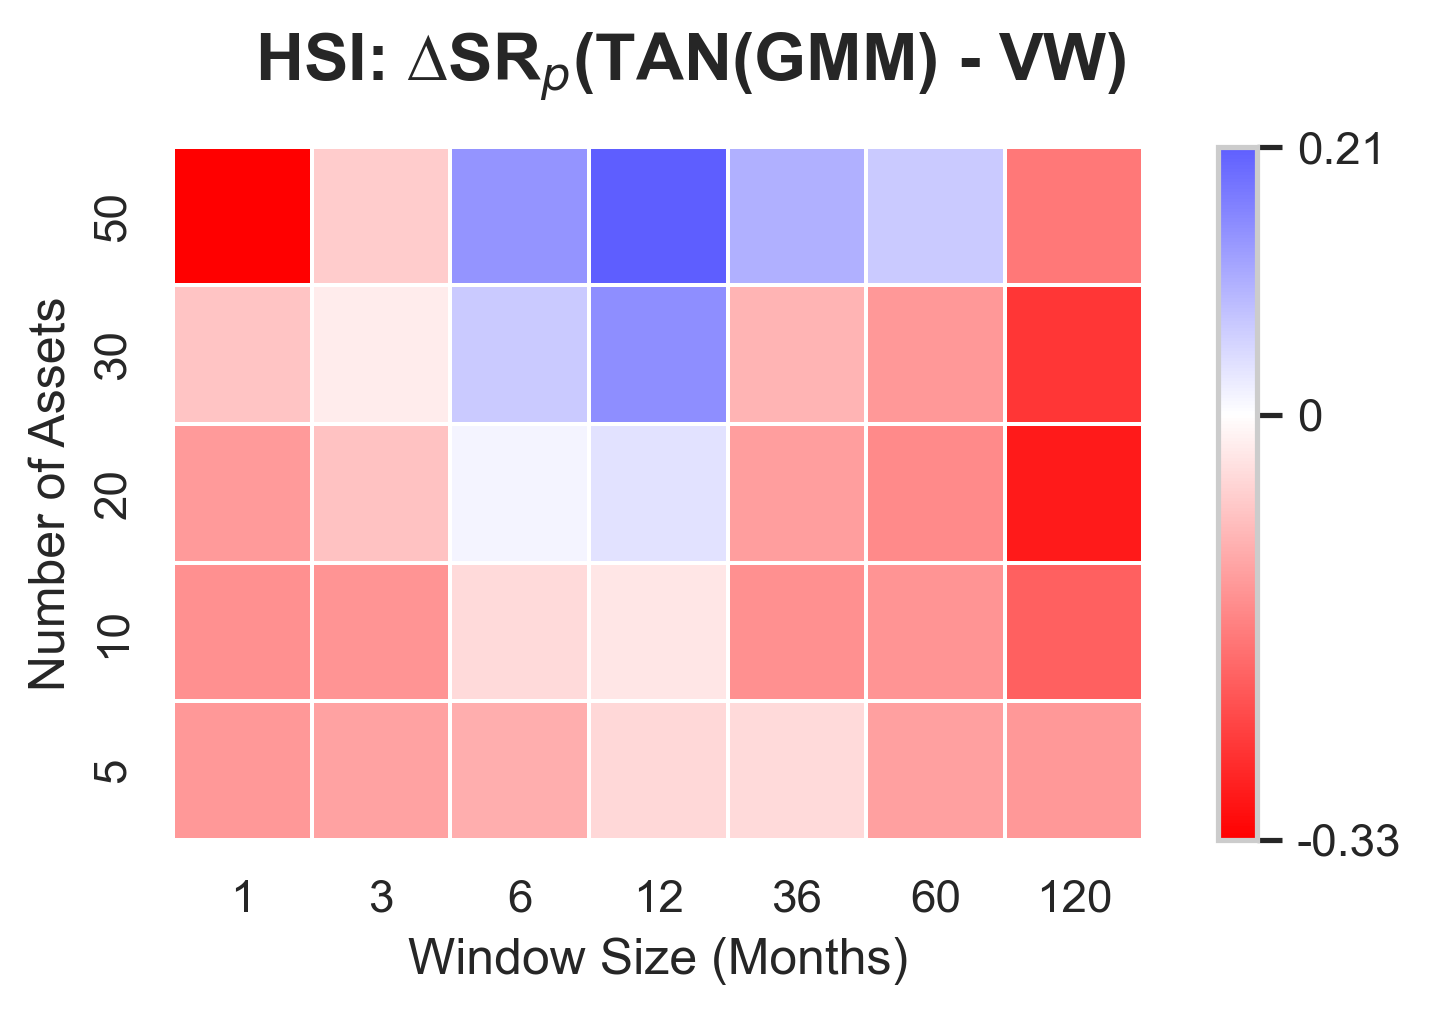
\includegraphics[width=0.5\textwidth]{images/40_18.png}
  \end{minipage}
  \caption[Heatmap 5]{Diverging-color heatmap of the penalized Sharpe-ratio difference $\Delta SR_p = SR_p(\mathrm{TAN(GMM)}) - SR_p(\mathrm{VW})$ across model configurations on the HSI index. Otherwise identical to Figure \ref{fig:combined13}.}
  \label{fig:combined17}
  \end{center}
  \end{figure}

All in all, KDE, especially KDE(TAN), can provide a repeatable enhancement over traditional benchmarks. KDE(TAN) is preferable to TAN across most configurations. KDE is preferable to MAR when the investment universe is moderate ($N \lesssim 100$) and lookback windows are less than a year. Outside this configuration sweet spot, VW or MV remain the safer defaults. By contrast, GMM's high variance and narrow win regions render it unattractive in most scenarios. In the next section, we focus specifically on the KDE and TAN(KDE) portfolios.

\section{CART analysis}
While the heatmaps make it easy to spot the blue regions where the KDE portfolios add value, they do not translate those patches into operational rules. To turn the visual hints into explicit decision criteria, we now fit a set of shallow classification trees. Using the 828 stable configurations that survive our 10\% observation-to-asset filter, we train depth-3 CART models to predict whether a given density-based portfolio beats its benchmark (i.e., whether $\Delta SR_{p}>0$ or $\Delta DD>0$). The input features are data frequency, look-back window (in months), universe size N, and the index. Rebalancing frequency did not improve accuracy and was excluded. The trained tree accuracy ranges from 0.71 to 0.85, suggesting that the splits capture the general structure without overfitting. The results below are grouped by the comparison metric. Because the decision-tree diagrams are visually dense and add little incremental intuition once their verbal rules are stated, we place the full plots in Appendix \ref{app:decisiontrees}.

\newpage
\textbf{Penalized Sharpe Ratio:}
For $\Delta SR_{p}(\text{KDE} - \text{VW})$, KDE outperforms only in two specific regions. In the HSI, it wins when using daily or weekly data and windows between 6 and 12 months. In the STOXX50, the edge appears with monthly data, small universes ($N \le 25$), and 6 to 12 months windows. $\Delta SR_{p}$ is negative elsewhere.

When comparing TAN(KDE) to VW, the advantage holds when $N > 25$ and the lookback is between 6 and 60 months. The performance difference is highly negative in the FTSE100 for ultra-short windows (1-3 months), and negligible in HSI and STOXX when the universe is small.

Against classical TAN, the TAN(KDE) portfolios outperform when using daily or weekly data with $N \le 40$ and windows of 60 to 120 months. Some additional gains persist for $N > 75$ under weekly or monthly data, but they are smaller.

\textbf{Maximum Drawdown:}
For drawdown control, KDE outperforms MV when daily data and long windows (6-120 months) are used. If the data frequency is weekly or monthly, KDE requires a small universe ($N \le 25$) and short windows ($\le 12$ months) to offer any advantage.

TAN(KDE) shows the clearest improvement over MV in larger universes ($N > 75$) with windows of 36 months or more, using daily or weekly data. Monthly frequency removes the advantage unless $N \le 25$.

% \textbf{Conclusion}
\subsection{Practical Summary}
Across the same configuration grid, GMM does not add value. It wins in fewer than 14\% of cases and increases drawdowns in over 90\%. Its trees collapse to trivial structures that predict consistent underperformance. Thus, only KDE-type strategies, applied in the regimes above, offer a repeatable edge over traditional portfolios. Below is a rule of thumb checklist for practitioners wishing to select the appropriate strategy:

\begin{enumerate}
\item High Sharpe Ratio: TAN(KDE), monthly data, 6-60 month window, any index  
\item Control tail-risk in large universes: baseline KDE, daily data, 6-120 month window, $N > 25$ (avoid STOXX50)
\item Short return histories ($\le 12$ months): use KDE over MAR; choose TAN(KDE) if return is the priority over volatility
\item Outside these regimes: default to VW for higher returns, MV for lower risk
\end{enumerate}

\newpage
\section{Limitations \& Path for Future Work}
\label{sec:limitations}
This section provides an overview of the limitations acknowledged in Section \ref{sec:introlimitations}, alongside rationales and suggestions for future research.

The absence of a KDE and GMM minimum-variance benchmark arises from analytical complexities. Specifically, the risk aversion term embedded within the log-sum-exponent structure cannot be factored out easily. This precludes a straightforward analytical derivation of the minimum-variance portfolio, as the usual limit taken to derive it cannot be performed directly. While the most straightforward alternative would be a numerical optimization procedure that iteratively searches through various risk-aversion parameters until the lowest variance is achieved, such an approach lies beyond the scope of this analysis. That is not to say that a closed-form formulation does not exist, but we were unable to derive it in a reasonable time. Hence, the derivation and application of minimum-variance strategies remain avenues for future research.

Similarly, we have not modeled transaction costs or portfolio turnover explicitly due to the practical infeasibility of doing so in the scope of exploring a large configuration space. Storing returns data alone required more than 40 GB of space; storing full weight timeseries for every configuration would have significantly increased the storage requirements further. Future studies may benefit from a targeted analysis of turnover and associated transaction costs.

In the main empirical analysis, we restricted KDE portfolios to strictly positive bandwidths ($H>0$). Ex-ante, this was prudent: a bandwidth of $H=0$ collapses the kernel to a discrete 'spike' density at each observation, which is mathematically consistent but prone to overfitting. Only after completing the out-of-sample evaluation did the visual inspection of portfolio frontiers (Section \ref{sec:frontier}) reveal that KDE's performance primarily arises from its adaptive weighting rather than smoothing effects. Thus, empirically validating the $H=0$ configuration emerges as a natural direction for future research.

Our choice of a 10\% observation-to-asset ratio cutoff for stable configurations was pragmatic, albeit based on ad-hoc considerations. Below that level, the training sample contains, on average, fewer than one year of monthly returns per asset, at which point all Markowitz-type strategies become numerically unstable and the resulting portfolios exhibit large swings in penalised Sharpe across seeds. Raising the threshold further removed only a few additional configurations, yet did not materially change any ranking of strategies, while lowering it to 5\% re-introduced the extreme S\&P500 outcomes that first alerted us to the problem. Thus, 10\% served as the smallest filter that eliminated the problematic cases without discarding a large portion of the configuration grid.

Our empirical analysis has focused on exploring a wide spectrum of portfolio strategies, but future research would benefit from a narrower focus on specific promising configurations. Additionally, the use of intraday data and explicitly examining market-timing strategies may prove to be insightful.

Finally, while KDE addresses the Markowitz assumption of normality, it leaves unchallenged the assumption of distributional stability over time. Significant value may be added by modeling temporal changes in distributions rather than static distributions. An accessible starting point, using only price data, would be integrating return forecasts from ARMA-GARCH models into the KDE framework.